\chapter{CÁC CÔNG TRÌNH LIÊN QUAN}

\section{Những phương pháp đã được sử dụng}

Định vị trực quan được định nghĩa là một bài toán nhằm xác định được vị trí của máy ảnh từ ảnh chụp được. Cho đến hiện tại, nhiều hướng tiếp cận cho bài toán định vị trực quan đã được đề xuất. Những phương pháp quan trọng nhất có thể được nhóm vào hai nhóm chính là \textbf{Những phương pháp sử dụng biểu diễn 3D} và \textbf{Những phương pháp hồi quy vị trí}. 

\begin{figure}[H]
    \centering
    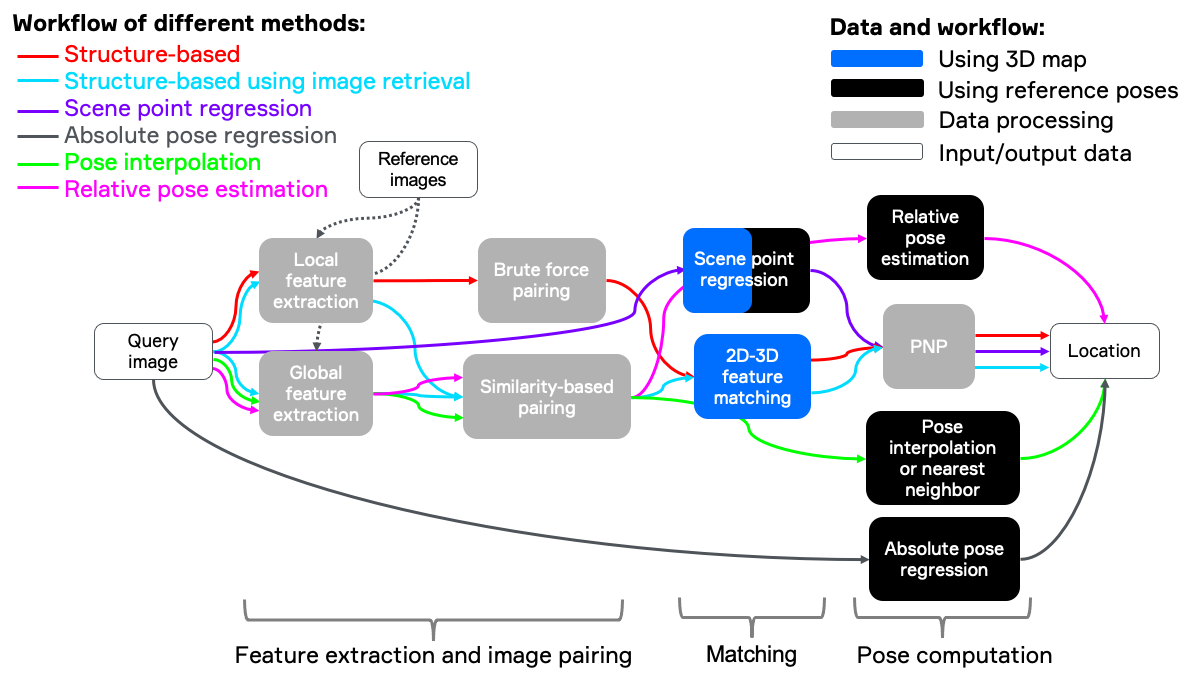
\includegraphics[scale=0.45]{pics/Chapter2/overviewViLoc.png}
    \caption{Tổng quát về những phương pháp định vị trực quan quan trọng \cite{methodsLocal}}
\end{figure}

\subsection{Những phương pháp sử dụng biểu diễn 3D}
\subsubsection*{Ý tưởng}
Những phương pháp sử dụng biểu diễn 3D sẽ hoạt động xoay quanh việc biểu diễn lại môi trường đang xét bằng một bản đồ đám mây điểm 3D. Bản đồ 3D chứa những đặc trưng trích xuất được từ các ảnh và tiến hành kiếm các cặp đặc trưng tương quan giữa các ảnh với nhau nhằm tạo thành những điểm mô tả 3D trong không gian ba chiều. Những bản đồ này thường sẽ được mô hình tạo ra vào lúc tiền xử lý tập dữ liệu và sẽ được dùng trong suốt quá trình bản địa hóa của mô hình.
\subsubsection*{Những bước thực hiện}
\begin{itemize}
    \item Ở bước tiền xử lý, không gian được thể hiện bởi tập dữ liệu sẽ được tái tạo lại trong không gian 3D, sử dụng những ảnh cùng thể hiện một cảnh, nhưng từ những vị trí và góc nhìn khác nhau. Phương pháp tái tạo này được gọi là Tái tạo kiến trúc từ chuyển động - Structure from Motion. Cụ thể hơn, quá trình này sẽ gồm các giai đoạn:
    \begin{itemize}
        \item Trích xuất mô tả của các đặc trưng từ ảnh: Mỗi ảnh trong tập dữ liệu sẽ được trích xuất đặc trưng và mỗi đặc trưng sẽ được gán một giá trị mô tả để SfM có thể tìm được những đặc trưng tương đồng giữa các hình. Kết quả đầu ra sẽ là một tập các mô tả cho đặc trưng của từng ảnh.
        \item Tìm kiếm sự tương quan của các đặc trưng giữa các ảnh: SfM sẽ tìm kiếm những ảnh cùng nhìn bộ phận của cảnh bằng cách kiểm tra sự tương đồng giữa các mô tả của đặc trưng trên các ảnh. Những cặp ảnh chứa những cặp đặc trưng tương quan sẽ cần được xác nhận lại về tính đúng đắn về hình học qua việc có tồn tại một cách biến đổi có khả năng ánh xạ một số lượng trưng giữa hai ảnh.
        \item Tái tạo lại cấu trúc: Quá trình tái tạo lại cấu trúc sẽ bắt đầu từ một cặp ảnh khởi tạo. Sau đó, không gian điểm 3D sẽ dần được mở rộng khi các ảnh được thêm tuần tự qua giải thuật PnP trong vòng lặp RANSAC.
    \end{itemize}
    \item Sau khi có được bản đồ đám mây điểm 3D biểu diễn môi trường đang xét, khi mô hình nhận vào một ảnh mới, những đặc trưng trong ảnh sẽ được trích xuất và so sánh mô tả của chúng với những điểm trong bản đồ 3D của khu vực. Khi những cặp đặc trưng 2D-3D đã được xác định, giải thuật PnP trong vòng lặp RANSAC sẽ được sử dụng một lần nữa để xác định vị trí của ảnh được chụp.
\end{itemize}
\subsubsection*{Những biến thể của phương pháp}

Một trong những tác vụ quan trọng nhất trong bài toán định vị bằng biểu diễn 3D chính là việc trích xuất ra được đặc trưng của ảnh và tạo cách mô tả thích hợp cho chúng. Ở những phương pháp truyền thống, những giải thuật được định nghĩa thủ công như SIFT \cite{lowe2004distinctive} và SURF \cite{bay2006surf} sẽ được sử dụng. Tuy nhiên, ở những giải thuật này tồn tại một số điểm yếu, xuất phát từ việc chúng không được thiết kế đặc biệt cho tác vụ hiện tại là truy xuất những ảnh biểu diễn cảnh giống nhau. Điều này sẽ làm giảm hiệu quả, đặc biệt trong điều kiện thay đổi như ngày-đêm, thay đổi theo mùa. Trong khoảng thời gian gần đây, những hướng tiếp cận theo hướng học sâu đã được đề xuất, chủ yếu sử dụng mạng CNN để trích xuất và biểu diễn đặc trưng. Những cách tiếp cận này vẫn gặp khó khăn trong việc nhận biết được những đặc điểm hình học trong hình \cite{zhou2020learn}.

Để có thể biểu diễn chính xác được một thành phố lớn trong không gian 3D, một lượng lớn điểm 3D sẽ cần được sử dụng. Với tập dữ liệu Aachen Day-Night \cite{sattler2018benchmarking}, mô hình 3D sẽ có số lượng điểm dao động từ 700 nghìn cho đến 2.5 triệu, tùy thuộc vào số lượng cặp ảnh được dùng. Vì vậy, chiến lược tìm kiếm Brute-Force sẽ dần trở nên bất khả thi khi môi trường biểu diễn trở nên lớn hơn. Để giới hạn lại không gian tìm kiếm, chiến lược truy xuất ảnh đã được sử dụng để tìm kiếm ảnh trong tập dữ liệu tương đồng nhất với ảnh truy vấn. Sau đó, việc tìm kiếm tương quan sẽ chỉ diễn ra trong không gian được thể hiện bởi những ảnh đó \cite{sarlin2019coarse}.

Để không phải lưu trữ một bản đồ 3D cho toàn khu vực đang xét, một phương pháp khác đã được đề xuất là xây dựng bản đồ điểm 3D cục bộ. Thay vì sinh ra bản đồ 3D cho toàn bộ khu vực đang xét ở bước tiền xử lý, phương pháp này sẽ sử dụng những ảnh truy xuất được để sinh ra bản đồ cục bộ \cite{sattler2017large}. Phương pháp này có thể tận dụng được những điểm mạnh của việc sử dụng cách biểu diễn 3D mà không cần duy trì bản đồ điểm 3D của toàn bộ khu vực. Tuy nhiên, cách tiếp cận này vẫn có một số điểm yếu như việc thời gian chạy trở nên đáng kể và số lượng ảnh truy xuất được có thể chưa đủ để sinh ra một bản đồ 3D phù hợp.

Một cách tiếp cận khác với mục tiêu loại bỏ sự cần thiết của bản đồ 3D, sử dụng mạng học sâu để xác định được vị trí của một điểm ảnh trong môi trường 3D, gọi là hồi quy điểm trong cảnh - Scene Point Regression \cite{brachmann2021visual}. Tuy nhiên, những mô hình thuộc phương pháp này không có tính khái quát hóa mà để có thể chạy trên một khu vực nhất định thì mô hình cần dữ liệu mẫu thuộc khu vực đó để huấn luyện.

\subsubsection*{Phân tích ưu và nhược điểm của phương pháp}
Nhờ vào việc sử dụng cách biểu diễn trong không gian 3D, lớp phương pháp này đã thành công học được tính hình học của môi trường, nhờ vậy nên những kết quả của lớp phương pháp này thường sẽ đạt được kết quả định vị chính xác. Ngoài ra, lớp phương pháp này sử dụng điểm 3D trong không gian làm mốc để định vị. Nhờ vậy nên mô hình vẫn sẽ cho ra được kết quả tốt khi không gian mẫu của vị trí chụp của ảnh bị giới hạn.

\begin{figure}[H]
    \centering
    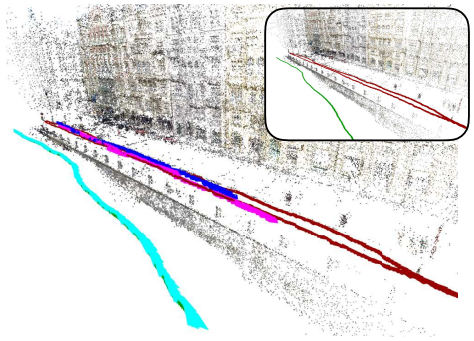
\includegraphics[scale=0.7]{pics/Chapter2/lim.png}
    \caption{Kịch bản khi mà tập dữ liệu huấn luyện bị hạn chế. Quỹ đạo của tập huấn luyện và tập kiểm thử có màu \textcolor{red}{đỏ} và \textcolor{green}{xanh lá}. Kết quả của những mô hình lấy vị trí của ảnh làm mốc là PoseNet \cite{kendall2016posenet} và MapNet \cite{brahmbhatt2018geometryaware} có quỹ đạo kết quả màu \textcolor{blue}{xanh dương} và \textcolor{purple}{tím}. Kết quả của phương pháp sử dụng biểu diễn 3D là Active Search \cite{sattler2016efficient} có quỹ đạo màu \textcolor{cyan}{xanh lam}}
\end{figure}

Đa số những vấn đề xoay quanh lớp phương pháp này sẽ liên quan đến việc sinh ra, lưu trữ và sử dụng biểu diễn 3D của khu vực. Do những bản đồ 3D biểu diễn những khu vực lớn sẽ có nhiều điểm 3D, dẫn đến việc tiêu tốn nhiều tài nguyên tính toán để sinh ra và sử dụng, đồng thời cần nhiều bộ nhớ để lưu trữ. Ngoài ra, đánh đổi cho khả năng biểu diễn một khu vực với độ chi tiết cao, những mô hình sử dụng cách biểu diễn 3D sẽ mất khả năng khái quát hóa khi xử lý những ảnh bên ngoài khu vực đang xét và cần phải được huấn luyện lại trên tập dữ liệu khác.

\subsection{Những phương pháp hồi quy vị trí}
\subsubsection*{Ý tưởng}
Với những thành công gần đây trong các tác vụ của ngành khoa học máy tính như phân loại ảnh, phân vùng ảnh theo ngữ nghĩa, truy xuất ảnh, những phương pháp sử dụng mạng học sâu đã có thể phần nào trích xuất được những thông tin hình học từ ảnh. Sử dụng những thông tin này, mô hình học sâu có thể xây dựng một hàm ánh xạ đến những cách biểu diễn mong muốn. Vì tính linh hoạt của hướng tiếp cận học sâu nên chúng có thể được ứng dụng để thay thế một hay nhiều tác vụ bên trong quá trình giải bài toàn định vị trực quan.
\subsubsection*{Những bước thực hiện}

Để những phương pháp học sâu có thể hoạt động một cách hiệu quả, mô hình cần được cung cấp một tập dữ liệu đã có kết quả để huấn luyện trên đó. Sau đó, mô hình học sâu có thể biến đổi dữ liệu đầu vào thành kết quả một cách trực tiếp, không cần sự can thiệp của con người. Cụ thể hơn, một phương pháp hồi quy vị trí sẽ thường có những bước sau:
\begin{itemize}
    \item Huấn luyện mô hình trên tập dữ liệu mẫu
    \item Xử lý dữ liệu đầu vào
    \begin{itemize}
        \item Mã hóa dữ liệu
        \item Ánh xạ tới cách biểu diễn phù hợp
    \end{itemize}
\end{itemize}
\subsubsection*{Những biến thể của phương pháp}

Hồi quy vị trí tuyệt đối

Hồi quy vị trí tương đối
\subsubsection*{Phân tích ưu và nhược điểm của phương pháp}

\subsection{Những phương pháp khác}
Viết phong long gì cũng được
\subsection{Xác định những vấn đề hiện hữu trong bài toán định vị trực quan}

\begin{itemize}
    \item \textbf{Những phương pháp hồi quy vị trí}
    \begin{itemize}
        \item Vấn đề về phạm vi hoạt động của mô hình: Đa số những mô hình hồi quy vị trí đều chỉ hoạt động tốt trên những tập dữ liệu có phạm vi nhỏ và phân bố dày đặc như 7Scenes \cite{6619221} và Cambridge Landmarks \cite{kendall2016posenet}. Đối với những tập dữ liệu có phạm vi rộng và phân bố thưa như Aachen Day-Night \cite{Sattler2012ImageRF}, chỉ phương pháp nội suy đơn giản đã được áp dụng và kết quả đem lại là không quá tốt.
        \item Vấn đề về khả năng khái quát hóa: Những mô hình hồi quy tuyệt đối sẽ xây dựng ngầm biểu diễn của khu vực đang xét bên trong những trọng số của mô hình. Vì vậy nên, một mô hình được huấn luyện trên một không gian nhất định chỉ có thể xử lý những ảnh được chụp trong không gian đó. Đối với những mô hình hồi quy tương đối, vấn đề này sẽ phụ thuộc vào cơ chế truy xuất ảnh được sử dụng.
        \item Vấn đề về độ chính xác: Những phương pháp hồi quy sẽ không cho ra kết quả chính xác như những phương pháp sử dụng cách biểu diễn 3D.
    \end{itemize}
    \item \textbf{Những phương pháp truy xuất ảnh}
    \begin{itemize}
        \item Vấn đề về tài nguyên xử lý: Tuy bài toán VPR đã có nhiều bước đột phá trong thời gian qua, đa số các phương pháp đạt kết quả tốt đều sử dụng những cách tổng hợp mô tả của các đặc trưng trong ảnh như NetVLAD \cite{arandjelović2016netvlad} hoặc những biến thể tích hợp cơ chế tập trung \cite{keetha2023anyloc}, ngữ nghĩa của bộ phận ảnh \cite{peng2021semantic}, bối cảnh của ảnh \cite{jin2017learned}. Những cơ chế đó sẽ có ảnh hưởng tiêu cực đến thời gian chạy do độ phức tạp của giải thuật cũng như độ lớn của không gian mô tả.
        \item Vấn đề về khả năng biểu diễn của CNN: Những cách tiếp cận theo mô hình học sâu sử dụng CNN cho đến hiện tại thường sẽ gặp những vấn đề trong việc biểu diễn được những thông tin về môi trường địa lý trong bài toán định vị trực quan.
    \end{itemize}
\end{itemize}

\section{Nhận dạng địa điểm trực quan - Visual Place Recognition}

Trước đây, việc định vị trực quan trên quy mô lớn (large-scale visual localization) được coi là một vấn đề truy xuất hình ảnh\cite{2022arXiv220105816X}. Vị trí cho hình ảnh truy vấn được xác định bởi hình ảnh tương tự nhất được lấy từ cơ sở dữ liệu. Tuy nhiên, để đáp ứng nhu cầu xác định vị trí của ảnh với độ chính xác trên 6 bậc tự do (6 Degrees of Freedom), việc sử dụng mô hình 3D để ước tính tư thế của máy ảnh ngày càng được các nhà nghiên cứu đề xuất và sử dụng. Sử dụng phương pháp này, bài toán định vị trực quan có thể được chia thành hai bước: truy xuất hình ảnh và định vị tư thế máy ảnh từ hình ảnh truy xuất được.

\subsection{Học biểu diễn - Representational learning}

\subsection{Học biểu diễn NetVLAD}

\subsection{Tối ưu hóa đặc trưng - MAC}

\subsection{Trung bình Hölder - Trung bình GeM}

\subsection{Truy xuất và tái xếp hạng}

\subsection{Học biểu diễn bằng Vision Transformer}

\subsection{Học biểu diễn bằng Feature Mixer}

\section{Ước tính vị trí của máy ảnh - Pose Estimation}

Ước tính vị trí máy ảnh (Camera Pose Estimation) là một bài toán thuộc chuyên ngành thị giác máy tính nhằm xác định vị trí (position) và góc quay (orientation) chính xác nhất có thể của máy ảnh thông qua dữ liệu hình ảnh được chụp từ chính máy ảnh. Đây là một bước cực kỳ quan trọng trong việc giải quyết bài toán định vị trực quan, thường được áp dụng sau khi bước nhận dạng địa điểm trực quan đã trích xuất được ảnh từ kho dữ liệu. Hiện nay, có tương đối nhiều hướng tiếp cận đối với bài toán này. Một trong những phương pháp phổ biến nhất là huấn luyện một mô hình học sâu để xác định 6 chiều tự do (Degree of Freedom) từ số ít ảnh (Absoblute Pose Regression và Relative Pose Regression) hoặc xây dựng một mô hình 3D từ tập dữ liệu có sẵn rồi tiến hành chuyển ảnh đầu vào sang các điểm 3D để dễ dàng so sánh và xác định vị trí (Structure From Motion).

\subsection{Hồi quy vị trí tuyệt đối - Absolute Pose Regression}

Hồi quy vị trí tuyệt đối (Absolute Pose Regression) hướng đến việc dự đoán vị trí và góc quay chính xác nhất của ảnh bằng một mô hình mạng nơ-ron tích chập thông qua việc cải thiện trọng số của mô hình. Tùy thuộc vào đầu vào của mô hình mà hồi quy vị trí tuyệt đối được chia thành ba hướng chính: hồi quy vị trí tuyệt đối với một ảnh, chuỗi ảnh hoặc đoạn phim.

\subsubsection*{Hồi quy vị trí tuyệt đối đơn ảnh - Absolute pose regression through single monocular image}
Với phương pháp hồi quy vị trí tuyệt đối thông qua một ảnh (Absolute pose regression through single monocular image), quy trình chung thường bao gồm: đầu vào - mạng - đầu ra. Đầu vào sẽ là một ảnh RGB với đầu ra là vị trí 6 độ tự do của máy ảnh. Thông thường, kiến trúc của mạng lưới tính toán sẽ bao gồm các thành phần như sau: bộ mã hóa, bộ định vị, bộ hồi quy. 

\begin{figure}[H]
    \centering
    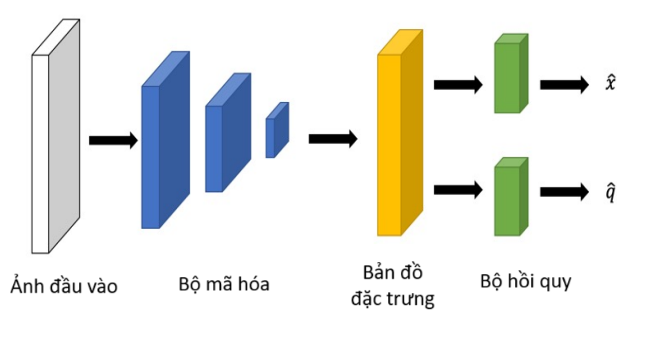
\includegraphics[scale=0.7]{pics/Chapter2/kientruc_APR_1.png}
    \caption{Kiến trúc mô hình hồi quy vị trí tuyệt đối đơn ảnh \cite{kendall2016posenet}}
\end{figure}

\noindent\textbf{Phương pháp sử dụng hàm mất mát Euclidean cố định:}

PoseNet \cite{kendall2016posenet} là công trình đầu tiên huấn luyện mô hình mạng nơ-ron tích chập để hồi quy vị trí máy ảnh từ một ảnh RGB, hoàn toàn không phụ thuộc vào bất kỳ cơ chế bên ngoài nào khác. Vào thời điểm ra mắt, PoseNet đã cho thấy sự vững chắc của mô hình vượt trội so với phương pháp tái tạo kiến trúc từ chuyển động dựa trên cơ chế "biến đổi tính năng bất biến tỷ lệ" (Scale-invariant Feature Transform Structure from Motion): độ hiệu quả của kiến trúc vế sau giảm mạnh nếu độ lớn của tập dữ liệu huấn luyện giảm đến một mức nhất định. Hàm mất mát Euclidean của PoseNet được định nghĩa như sau:
\begin{center}
$loss(I) = \left \| \hat{x} - x \right \|_2 + \beta \left \| \hat{q} - \frac{q}{\left \| q \right \|} \right \|_2$
\end{center}

Kế thừa từ PoseNet, đã có nhiều công trình và bài báo tìm cách cải thiện phương pháp định vị hoặc thay thế hàm mất mát nhằm nâng cao hiệu suất chung của toàn kiến trúc. Với các công trình có mong muốn cải thiện hàm mất mát của mô hình, một chiến thuật chung là kết hợp hàm mất mát Euclidean và phương pháp giảm độ dốc Stochastic. Về mặt cải thiện hiệu quả định vị cũng như tìm hiểu về độ thiếu chính xác của mô hình, một nhóm tác giả đề xuất thêm xác suất Bernoulli vào mô hình nơ-ron tích chập \cite{kendall2016modelling} nhằm xác định độ thiếu chính xác của mô hình. Ý tưởng chính của phương pháp này là xác định và tận dụng độ thiếu chính xác để dự đoán sai số trong định vị, phương pháp này đã cải thiện độ chính xác cho PoseNet cho cả những cảnh ngoài trời và bên trong nhà.
\begin{figure}[H]
    \centering
    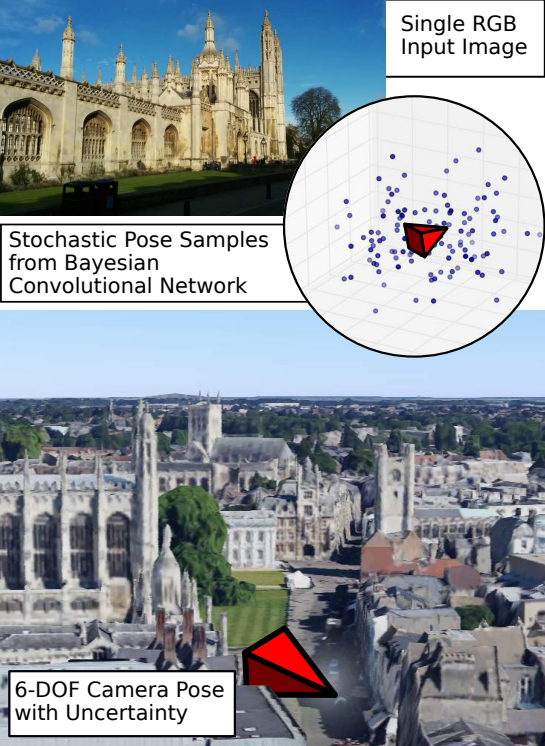
\includegraphics[scale=0.7]{pics/Chapter2/Ber_PoseNet.png}
    \caption{Minh họa mô hình CNN được áp dụng phân phối Bernoulli \cite{kendall2016modelling}}
\end{figure}
Từ những thông tin được nêu ra trong bài báo \cite{kendall2016posenet}, ta biết được rằng mô hình PoseNet có một lớp kết nối đầy đủ với 2048 chiều, tạo điều kiện cho việc áp dụng một lớp bộ nhớ dài ngắn hạn để giảm chiều đặc trưng giúp cải thiện độ chính xác định vị \cite{walch2017imagebased, wang2019atloc}. Nhóm tác giả Watch và cộng sự \cite{walch2017imagebased} đề xuất tận dụng các lớp bộ nhớ dài ngắn hạn lên đầu ra của PoseNet để giảm chiều và chọn ra những đặc trưng hữu ích nhất cho bài toán định vị vị trí. Các thí nghiệm đo lường cho thấy phương pháp này vượt trội hơn PoseNet khoảng 30\% về sai số vị trí và 55\% về sai lệch góc quay.
\begin{figure}[H]
    \centering
    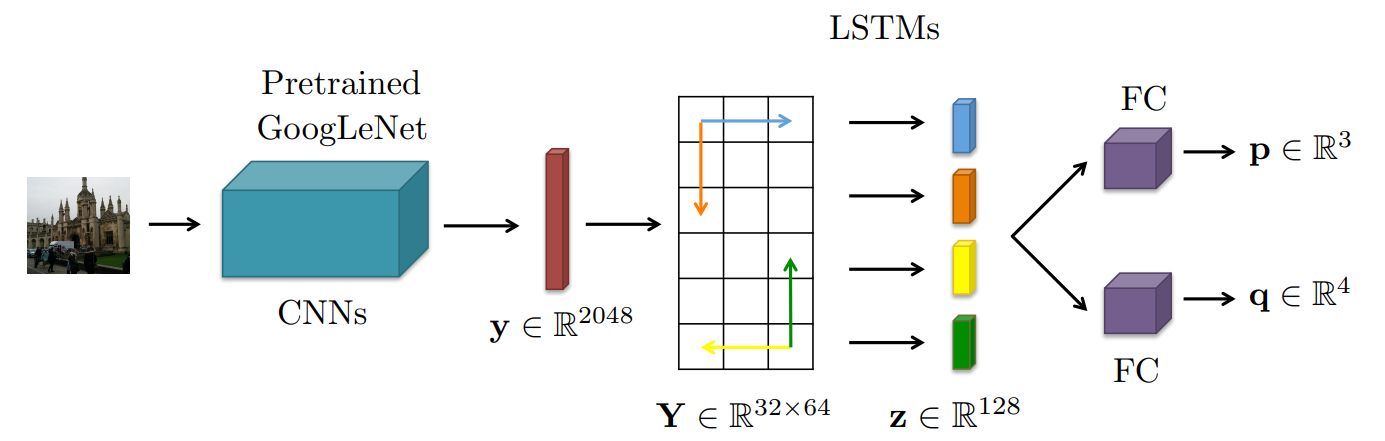
\includegraphics[width=\textwidth]{pics/Chapter2/LSTM_PoseNet.png}
    \caption{Minh họa kiến trúc mô hình LSTM PoseNet \cite{walch2017imagebased}}
\end{figure}
Để cải thiện độ chính xác định vị, một kiến trúc đồng hồ cát được đề xuất với việc thêm một phần chức năng mã hóa thông tin hữu ích từ kiến trúc vật thể thô và một phần chức năng thu chi tiết vật thể mịn. Hourglass PoseNet \cite{melekhov2017imagebased} có kiến trúc gồm ba thành phần chính là bộ mã hóa, bộ giải mã và bộ hồi quy. Mô hình này sử dụng một mô hình ResNet34 đã được tinh chỉnh làm bộ mã hóa - giải mã. SVS PoseNet \cite{inproceedings} dùng mô hình VGG16 kết hợp thêm hai lớp kết nối đầy đủ để có thể dự đoán riêng vị trí và góc quay. BranchNet \cite{7989663} sử dụng mô hình mạng hai nhánh học đồng thời biểu diễn góc quay và độ dời để giảm thiểu độ thưa của các vị trí được lấy mẫu một cách hiệu quả. Dù hướng tiếp cận có sự khác biệt, các công trình trên đều có cùng hàm mất mát với PoseNet.
\begin{figure}[H]
    \centering
    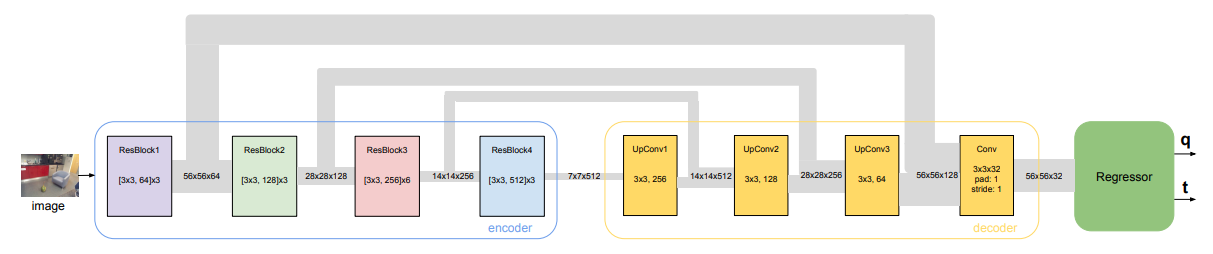
\includegraphics[width=\textwidth]{pics/Chapter2/hourglass_PoseNet.png}
    \caption{Minh họa kiến trúc mô hình Hourglass PoseNet \cite{melekhov2017imagebased}}
\end{figure}

\noindent\textbf{Phương pháp sử dụng hàm mất mát có trọng số học được:}

Để học được thông tin về vị trí và góc quay từ dữ liệu ảnh, hàm mất mát cố định Euclidean áp dụng các siêu tham số cân bằng để giúp việc học thông tin vị trí và góc quay một cách độc lập, tuy nhiên để học trọng số thì rất tốn kém. Geometric PoseNet \cite{kendall2017geometric} đề xuất sử dụng hàm mất mát vị trí có trọng số học được để cân bằng hiệu suất và cải thiện độ ổn định. Khi so sánh với PoseNet, phương pháp này giữ lại độ mở rộng và độ chắc chắn mà không cần chỉnh sửa các siêu tham số cố định cân bằng trong hàm mất mát. 

AtLoc \cite{wang2019atloc} thêm vào mô hình một mô-đun tập trung (Attention Module) trước khi xác định các tọa độ hồi quy để ép buộc mạng phải tập trung vào phần chính - phần mang nhiều thông tin hữu ích nhất của hình ảnh đầu vào. Ngoài ra, AtLoc sử dụng ResNet34 được huấn luyện sẵn trên tập dữ liệu ImageNet làm bộ mã hóa, sau đó hồi quy lớp kết nối đầy đủ 2048 chiều của PoseNet. 
\begin{figure}[H]
    \centering
    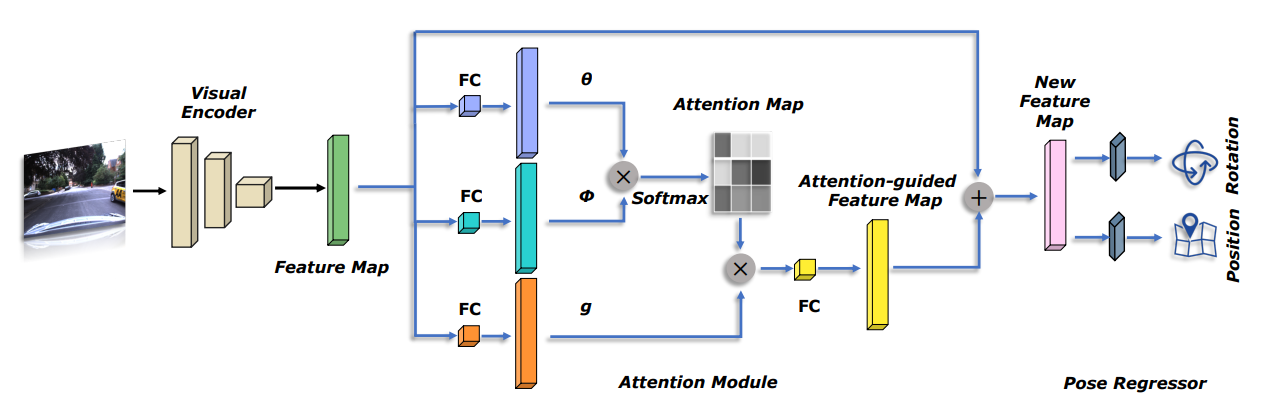
\includegraphics[width=\textwidth]{pics/Chapter2/atloc.png}
    \caption{Minh họa kiến trúc mô hình AtLoc \cite{wang2019atloc}}
\end{figure}
AdPR \cite{bui2019adversarial} thêm một mạng phân biệt và học đối lập. Điều này không chỉ hồi quy vị trí mà còn tinh chỉnh vị trí. Khi trích xuất đặc trưng, AdPR áp dụng mạng ResNet-18, vì nó có thể đạt được hiệu suất tốt nhất so với VGG16 và AlexNet. APANet \cite{chidlovskii2020adversarial} cũng sử dụng một mạng đối lập để tạo ra hình ảnh liên quan đến hình ảnh đầu vào để ước lượng tốt hơn vị trí của máy ảnh. Một mô-đun Dropout được thêm trước bộ mã hóa trích xuất đặc trưng để xuất ra nhiều khả năng không chắc chắn, điều này có thể cải thiện độ chắc chắn của mô hình dưới điều kiện thử thách như thay đổi vị trí, thời tiết,... . Sau khi trích xuất, mô-đun tập trung tự động được thêm để điều chỉnh lại trọng số bản đồ đặc trưng.
\begin{figure}[H]
    \centering
    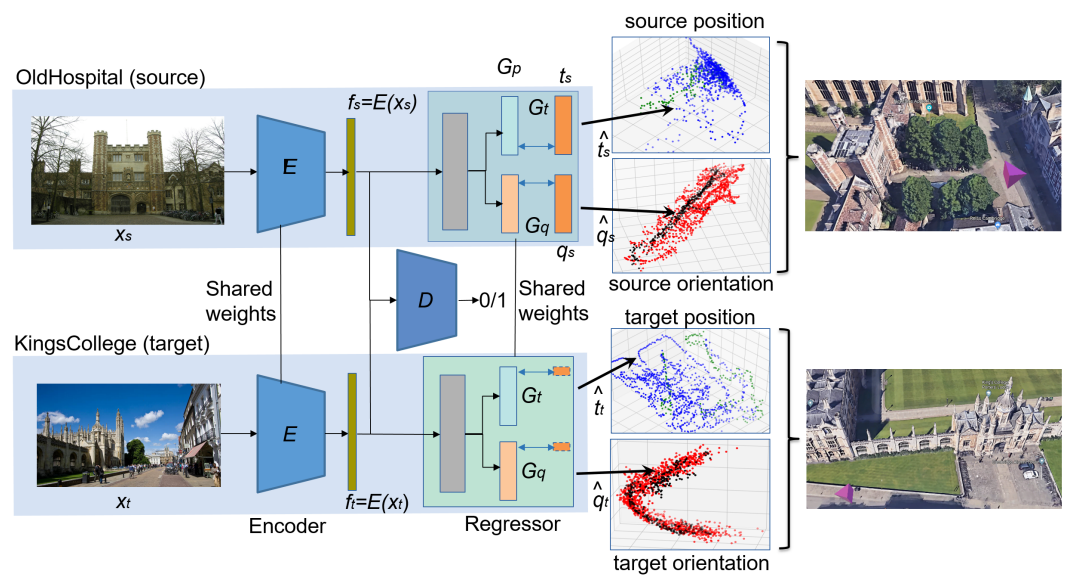
\includegraphics[width=\textwidth]{pics/Chapter2/apanet.png}
    \caption{Minh họa kiến trúc mô hình APANet \cite{chidlovskii2020adversarial}}
\end{figure}
\noindent\textbf{Phương pháp sử dụng hàm mất mát khác:}

Không dùng đến cả hàm mất mát cố định hoặc những hàm mất mát có trọng số học được, một số nhóm nghiên cứu đề xuất nên cân nhắc sử dụng các mô-đun khác để cải thiện hiệu suất định vị. GeoPoseNet \cite{kendall2017geometric} đề xuất sử dụng hàm mất mát tái chiếu: đặc tả sai sót tái chiếu của cảnh. Hàm mất mát tái chiếu chuyển mất mát chung học được thành khác biệt tọa độ ảnh, do đó có thể thay đổi trọng số giữa vị trí và góc quay, tùy thuộc vào các cảnh khác nhau trong quá trình huấn luyện mô hình. GPoseNet \cite{Cai2018AHP} xây dựng mô hình mới bằng cách thêm vào hai bộ "Hồi quy quá trình Gaussian suy luận biến phân ngẫu nhiên" (Stochastic Variational Inference Gaussian Process Regressions - SVI GPs) sau lớp kết nối đầy đủ để học phân phối xác suất của vị trí - hướng quay đầu ra và giảm tần suất sử dụng siêu tham số. Hàm mất mát của GPoseNet kết hợp hàm mất mát SVI GPs sử dụng ranh giới điều kiện dưới của hai xác suất tích lũy log $L_{s}vi$ và hàm mất mát CNN với siêu tham số $\beta_{g_{t}}$ và $\beta_{n_{q}}$ của PoseNet.
\begin{figure}[H]
    \centering
    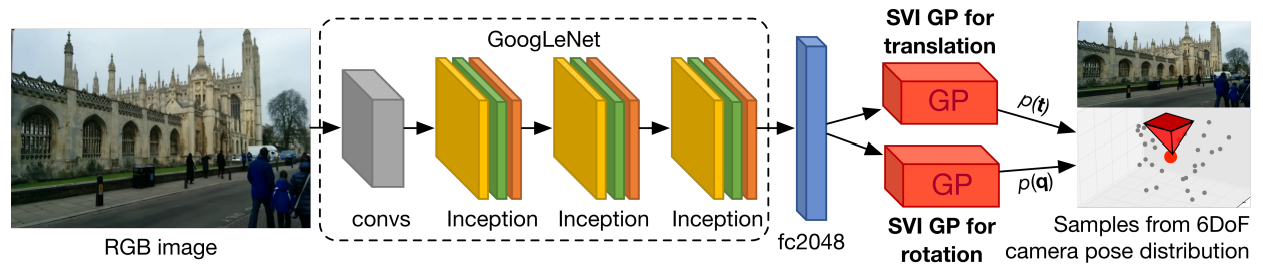
\includegraphics[width=\textwidth]{pics/Chapter2/gposenet.png}
    \caption{Minh họa kiến trúc mô hình GPoseNet \cite{kendall2017geometric}}
\end{figure}

Một nhóm nghiên cứu \cite{shavit2021learning, article} đề xuất áp dụng mô hình Transformer vào tác vụ hồi quy vị trí tuyệt đối. Mô hình nhận vào một ảnh đơn và sử dụng một CNN làm bộ trích xuất đặc trưng, sau đó các bản đồ đặc trưng được truyền song song qua hai nhánh: mỗi nhánh là một mô hình Transformer đảm nhiệm một tác vụ riêng lần lượt là hồi quy vị trí và hồi quy hướng quay. Mô hình sử dụng hàm mất mát tương tự với PoseNet.
\begin{figure}[H]
    \centering
    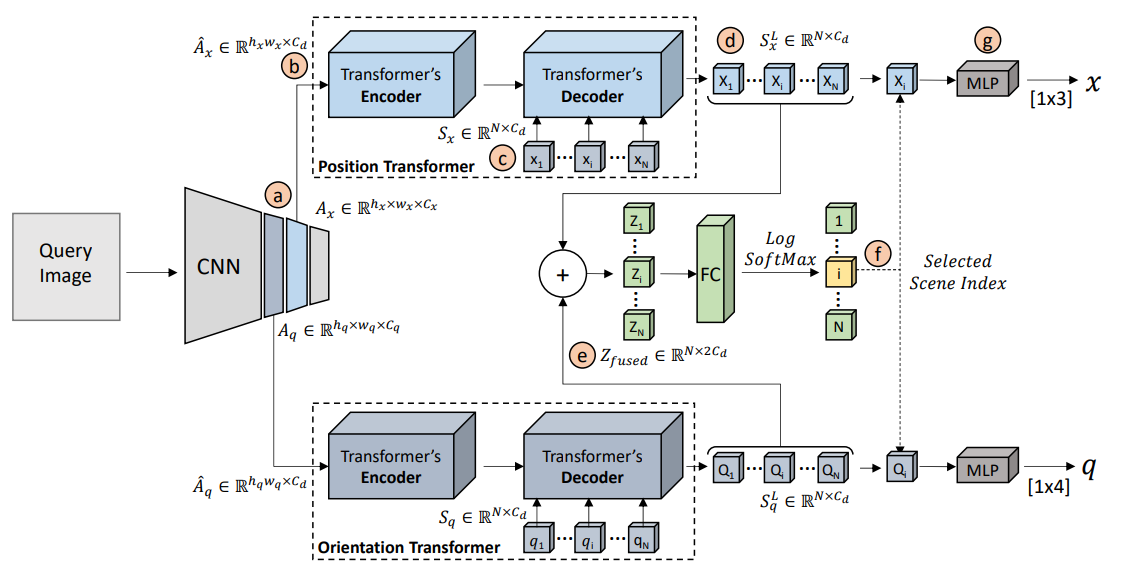
\includegraphics[width=0.7\textwidth]{pics/Chapter2/trans.png}
    \caption{Minh họa kiến trúc mô hình Multi-Scene Transformer \cite{shavit2021learning, article}}
\end{figure}

\subsubsection*{Hồi quy vị trí tuyệt đối đa ảnh - Absolute pose regression through auxiliary image sequence}
Một phương pháp khác được áp dụng để hồi quy vị trí tuyệt đối là áp dụng học có hỗ trợ với một chuỗi ảnh. Học có hỗ trợ được định nghĩa là phương pháp cải thiện hiệu suất của một tác vụ chính thông qua việc học cùng lúc các tác vụ hỗ trợ. Phương pháp học này giúp mô hình phát triển các biểu diễn dữ liệu tốt hơn. Bằng cách tận dụng các tác vụ hỗ trợ có liên quan khác trong quá trình học, hiệu suất của tác vụ chính có thể được cải thiện. Ở đây, học có hỗ trợ ám chỉ việc kết hợp APR với các tác vụ phụ có liên quan như đo lường cảm biến trực quan. Hàm mất mát của các phương pháp học có hỗ trợ thường bao gồm hàm mất mát của APR kết hợp với hàm mất mát của các phương pháp phụ trợ, thậm chí có thể kết hợp cả hàm mất mát của APR và RPR. Khác với các phương pháp hồi quy vị trí tuyệt đối đơn ảnh, phương pháp học có hỗ trợ học từ các cặp ảnh với bản chất là học cách xác định vị trí tuyệt đối bằng cách đánh giá trước hết vị trí tương đối với các ràng buộc phụ thuộc.

MapNet \cite{brahmbhatt2018geometryaware} đề xuất thêm một thuật ngữ mất mát lấy từ các cặp ảnh làm một ràng buộc hình học, điều này đã có thể cải thiện mạnh mẽ hiệu suất khả năng định vị. Về hàm mất mát, MapNet giảm thiểu tối đa cả mất mát vị trí tuyệt đối cho mỗi hình ảnh và mất mát vị trí tương đối giữa các cặp hình ảnh:
\begin{center}
    $l(I_{total}) = l(I_i) + \alpha\sum_{i\neq j}loss(I_{ij} )$
\end{center}
Trong đó, $loss(I_{ij} )$ ám chỉ vị trí máy ảnh tương đối $p_i$ và $p_j$ giữa các cặp hình ảnh $I_i$ và $I_j$, được tính bởi hàm mất mát với trọng số có thể học được.

Thêm vào đó, MapNet chuyển một giá trị quaternion thành logarit của giá trị đó - biểu diễn phép quay ba độ tự do (3DoF) với ba chiều chưa bị tham số hóa quá mức. $logq$ được biểu diễn như dưới đây, với $u$ và $v$ đại diện cho phần thực và ảo của một quaternion đơn vị:
\begin{center}
    $logq = 
    \begin{cases}
      \frac{v}{\left \| v \right \|}cos^{-1}u, \left \| v \right \| \neq 0\\    
      0   
    \end{cases}$
\end{center}
\begin{figure}[H]
    \centering
    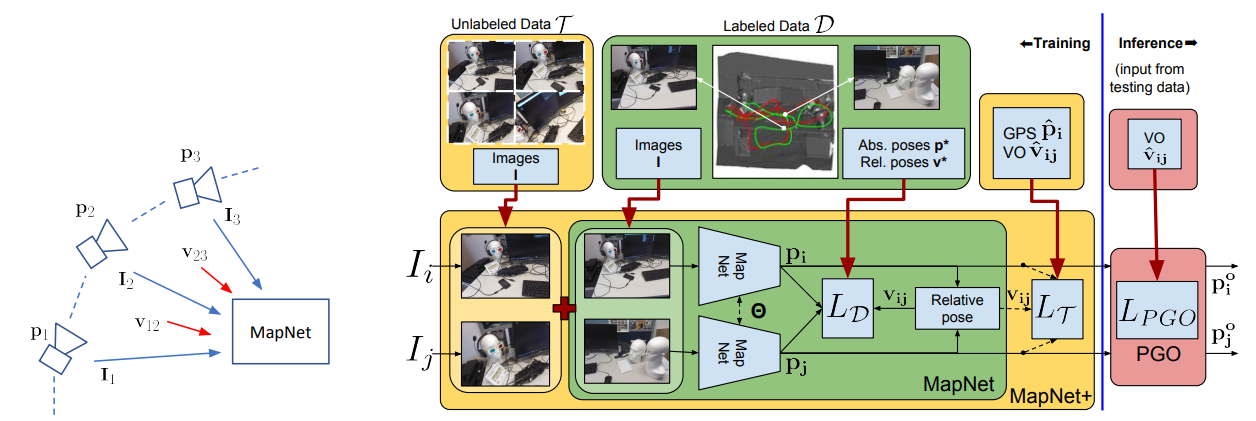
\includegraphics[width=\textwidth]{pics/Chapter2/mapnet.png}
    \caption{Minh họa kiến trúc mô hình MapNet \cite{brahmbhatt2018geometryaware}}
\end{figure}
Năm 2019, tác giả Xue và những cộng sự \cite{xue2019local} cũng có một hướng tiếp cận tương tự khi hồi quy vị trí máy ảnh thông qua những ràng buộc về không gian - thời gian, trong đó đặc trưng cục bộ cải thiện định vị toàn cục - gọi là "Cục bộ hỗ trợ toàn cục" (Local Support Global - LSG). Thêm vào đó, LSG đề xuất sử dụng một đánh giá đã được “tăng cường nội dung” để ước lượng lỗi vị trí và tinh chỉnh dựa trên chuyển động, để tối ưu hóa dự đoán vị trí thông qua các ràng buộc chuyển động. LSG sử dụng một hàm mất mát vị trí toàn cầu $L_g$ lấy từ hồi quy tuyệt đối, hàm mất mát hồi quy đo lường cảm biến trực quan $L_{vo}$, các ràng buộc hình học và hàm mất mát liên kết chuyển động $L_{joint}$ để tối ưu hóa hồi quy vị trí như sau:
\begin{center}
$l_{total} = l_g + l_{vo} + l_{joint}$
\end{center}
\begin{figure}[H]
    \centering
    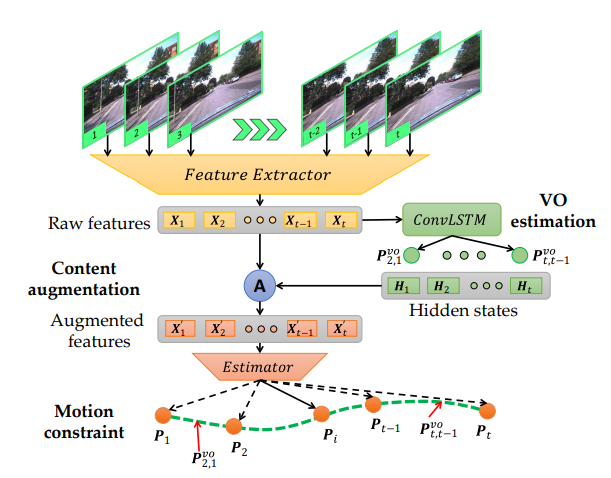
\includegraphics[width=0.5\textwidth]{pics/Chapter2/lsg.png}
    \caption{Minh họa kiến trúc mô hình LSG \cite{xue2019local}}
\end{figure}
VlocNet \cite{valada2018deep} cũng học đồng thời đo lường cảm biến trực quan như một tác vụ phụ để hồi quy vị trí toàn cục với hai mạng phụ. Mất mát nhất quán hình học được điều chỉnh để giảm thiểu tối đa lỗi vị trí, được định nghĩa như sau:
\begin{center}
$l(I_{total}) = (I_{i_x} + I_{ij_x})exp(-\hat{s}_x) + (I_{i_q} + I^{q}_{ij})exp(-\hat{s}_q)+ \hat{s}_q$
\end{center}
\begin{figure}[H]
    \centering
    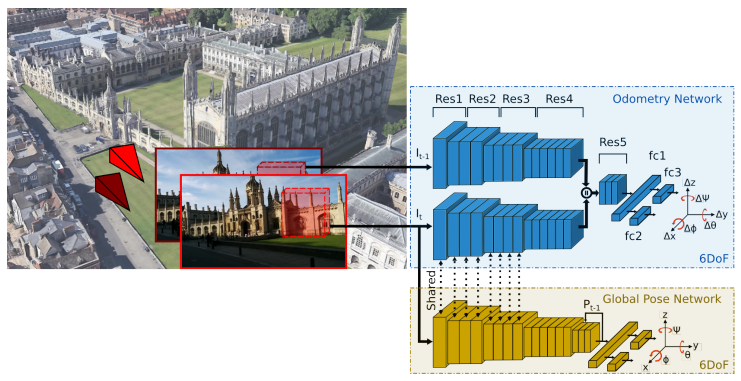
\includegraphics[width=0.7\textwidth]{pics/Chapter2/vlocnet.png}
    \caption{Minh họa kiến trúc mô hình VlocNet \cite{valada2018deep}}
\end{figure}
VlocNet++ \cite{Radwan_2018} giới thiệu kiến thức ngữ nghĩa vào hồi quy vị trí, kết hợp thông tin hình học-thời gian với các đặc trưng ngữ nghĩa cùng một lúc. Hàm mất mát của VlocNet++ kết hợp hồi quy vị trí toàn cục, mất mát đo lường cảm biến trực quan và mất mát Entropy chéo cho mất mát phân đoạn ngữ nghĩa cùng một lúc, với ba yếu tố $\hat{s}_{log}$, $\hat{s}_{vo}$ và $\hat{s}_{seg}$ để cân bằng ba thành phần này:
\begin{center}
$ l(I_{total}) = l_{loc}exp(-\hat{s}_{loc})+ \hat{s}_{loc}+l_{vo}exp(-\hat{s}_{vo})+ \hat{s}_{vo}+l_{seg}exp(-\hat{s}_{seg})+ \hat{s}_{seg}$
\end{center}
\begin{figure}[H]
    \centering
    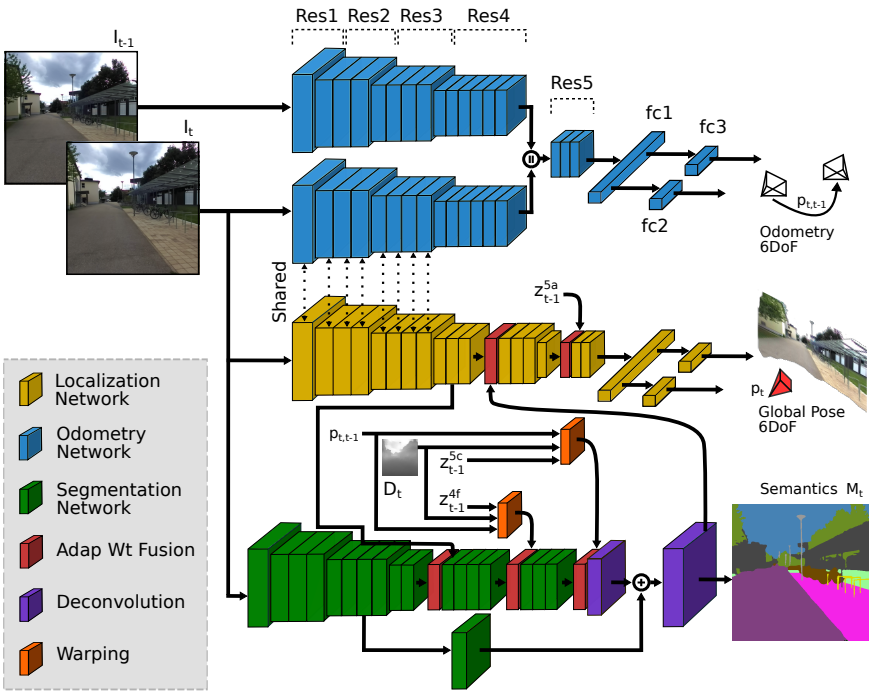
\includegraphics[width=0.7\textwidth]{pics/Chapter2/vlocnetplus.png}
    \caption{Minh họa kiến trúc mô hình VlocNet++ \cite{Radwan_2018}}
\end{figure}
Một bản mở rộng của AtLoc, AtLocPlus \cite{wang2019atloc} cũng kết hợp các ràng buộc thời gian để học cùng lúc mất mát vị trí tuyệt đối và mất mát vị trí tương đối, dẫn đến hiệu suất tốt hơn AtLoc trong việc sử dụng một đầu vào ảnh đơn. AtLocPlus sử dụng hàm mất mát giống với MapNet.

DGRNet \cite{lin2019deep} đề xuất một kiến trúc với một mạng con hồi quy vị trí tương đối RCNN1, một mạng con hồi quy vị trí toàn cục RCNN2 và lớp kết hợp kết nối đầy đủ dùng để trích xuất đặc trưng từ ảnh. Ràng buộc biến đổi chéo (Cross transformation constraint – CTC) và sai số toàn phương trung bình (Mean squared error – MSE) được áp dụng vào hàm mất mát để cải thiện hiệu suất hồi quy. DGRNet đã sử dụng kết hợp hàm mất mát tương đối, toàn cục, CTC $\hat{l}_i$ và sự thật nền tảng $\hat{P}_i$ như sau:
\begin{center}
$ w = \underset{w}{argmin} \frac{1}{N}^{N}_{i=1} \sum_{k=0}^{6}(l^i_k) + \sum_{j=0}^{4}\left \| P^ij - \hat{P}^i_j \right \|^2_2 $
\end{center}
\begin{figure}[H]
    \centering
    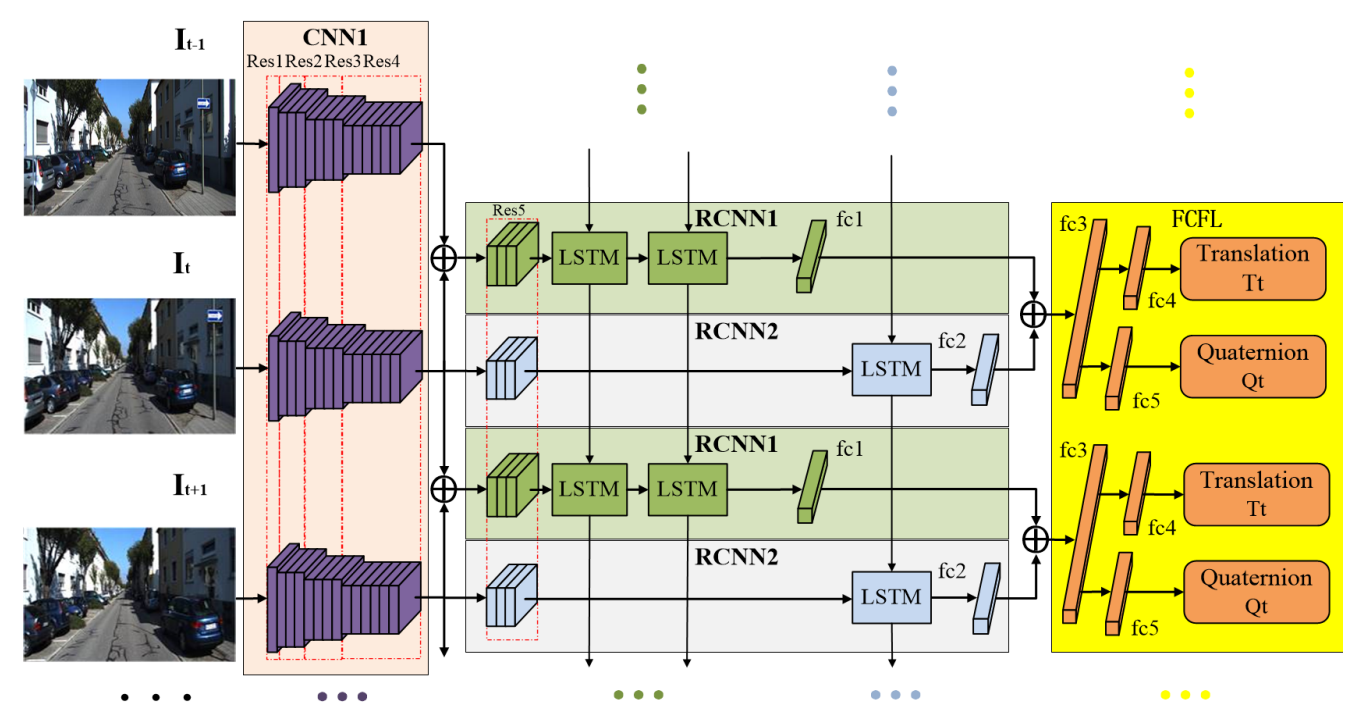
\includegraphics[width=0.7\textwidth]{pics/Chapter2/dgrnet.png}
    \caption{Minh họa kiến trúc mô hình DGRNet \cite{lin2019deep}}
\end{figure}
\subsubsection*{Hồi quy vị trí tuyệt đối qua đoạn phim - Absolute pose regression through video}

Không chỉ đơn ảnh hay đa ảnh, ngay cả đoạn phim cũng có thể được sử dụng để thêm một ràng buộc thời gian có tính trơn tru hơn cho hồi quy vị trí. Các đoạn phim hay các dữ liệu cảm biến khác đều có thể được truy cập dễ dàng bởi các thiết bị di động. Đoạn phim có thể được đồng bộ hóa với các dữ liệu đầu vào khác như đo lường cảm biến trực quan, các cảm biến IMU như đồng hồ tăng tốc và đồng hồ quay và dữ liệu GNSS bằng thông tin thời gian , cụ thể là bằng cách căn chỉnh các mốc thời gian. Với một quy trình tương tự như các phương pháp ARP dựa trên hình ảnh đơn và chuỗi hình ảnh, ARP dựa trên đoạn phim cũng hồi quy độ dời và hướng quay thông qua bộ trích xuất đặc trưng là một mạng nơ-ron tích chập và bộ hồi quy vị trí cục bộ.

VidLoc \cite{clark2017vidloc} đề xuất một mô hình hồi quy vị trí máy ảnh dựa trên việc kết hợp CNN – RNN, mục đích là có thể khiến quá trình dự đoán vị trí từ ảnh hay một đoạn phim được trơn tru hơn. Mạng được xây dựng bằng cách sử dụng GoogLeNet Inception \cite{szegedy2014going} mà không dùng đến lớp kết nối đầy đủ để trích xuất đặc trưng ảnh và một mô-đun LSTM hai chiều để mô hình hóa thông tin thời gian với các ô nhớ.  Hàm mất mát của VidLoc được tính bằng tổng của lỗi vị trí và lỗi hướng quay từ đầu ra của LSTM như sau:
\begin{center}
$ l = \sum_{t=1}^T \alpha_1 \left \| x_t - \hat{x}_t \right \| + \alpha_2 \left \| q_t - \hat{q}_t \right \| $
\end{center}
Với $[x_t, q_t]$ và $[\hat{x}_t, \hat{q}_t]$ đại diện cho sự thật nền tảng và giá trị dự đoán cho độ dời vị trí và hướng quay.
\begin{figure}[H]
    \centering
    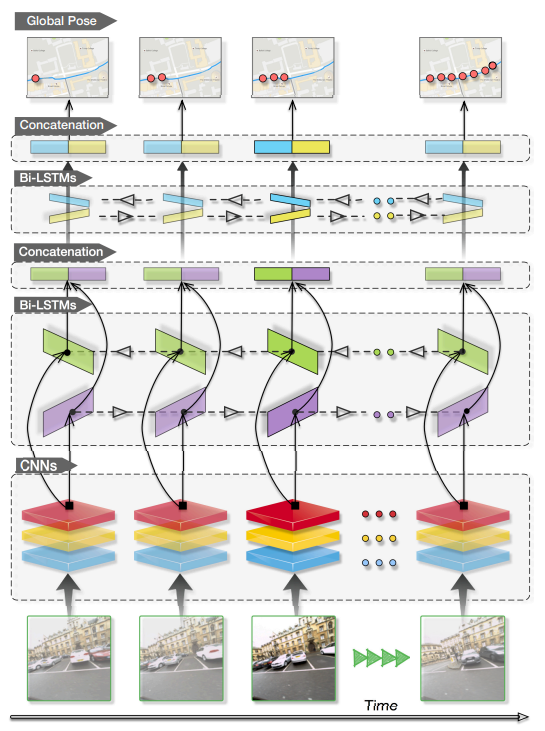
\includegraphics[width=0.7\textwidth]{pics/Chapter2/vidloc.png}
    \caption{Minh họa kiến trúc mô hình VidLoc \cite{clark2017vidloc}}
\end{figure}
MapNet+ và MapNet+PGO \cite{brahmbhatt2018geometryaware} mang cùng một kiến trúc mạng với MapNet trích xuất đặc trưng qua mạng ResNet34 và dùng một lớp tổng hợp trung bình toàn cục. Không chỉ dùng mất mát vị trí tuyệt đối, mất mát đo lường cảm biến trực quan cũng được tính toán để cải thiện hiệu suất dự đoán vị trí của MapNet. Phương pháp này cũng đồng thời tích hợp dữ liệu GNSS và IMU để giúp cải thiện hồi quy vị trí. Điều này giúp kết hợp dữ liệu đã được gắn nhãn và dữ liệu chưa gắn nhãn từ VO hay cảm biến để phục vụ cho việc học tự giám sát và đã thể hiện hiệu suất tốt dưới những điều kiện khó khăn, thử thách như thay đổi môi trường ngoài, thiếu sáng,... .
\begin{center}
$l = l_{labelled data} + l_{unlabelled data}$
\end{center}
Với mất mát từ dữ liệu chưa gắn nhãn có thể được tính toán thông qua việc kết hợp vị trí máy ảnh tương đối $v_ij$ và VO $\hat{v}_ij$ hay các cảm biến khác như IMU và GNSS. 

MapNet+PGO đã có thể cải thiện hiệu suất đồng thời giảm thiểu chi phí tính toàn thông qua việc sử dụng cải thiện đồ thị vị trí (PGO) để kết hợp kết quả vị trí MapNet+ và VO.

\subsubsection*{Kết luận}
Xét về các phương pháp mang hướng hồi quy vị trí tuyệt đối thông qua một ảnh duy nhất, các nghiên cứu có xu hướng tiến tới việc hàm mất mát tự động hóa, không sử dụng siêu tham số và mang nhiều thông tin hơn để giảm việc sử dụng các tham số cố định. Khởi đầu từ PoseNet với việc sử dụng một hàm mất mát cố định để tính tổng độ dời và hướng quay sử dụng một số tham số cân bằng. Sau đó, một hàm mất mát có trọng số học được \cite{wang2019atloc, bui2019adversarial} đã được đề xuất bằng cách thêm độ không đảm bảo phương sai đồng nhất để tự động cân bằng mất mát độ dời và hướng quay, tránh sử dụng siêu tham số đồng thời vượt qua hiệu suất của phương pháp sử dụng hàm mất mát cố định. Ngoài phương pháp hàm mất mát cố định và hàm mất mát với trọng số học được, một số công trình \cite{kendall2017geometric, Cai2018AHP} đề xuất sử dụng mất mát lỗi tái chiếu và mất mát GPoseNet để thêm các định dạng thông tin khác như phân phối xác suất của vị trí - hướng quay đầu ra để cải thiện hàm mất mát. 

Với việc sử dụng nhiều ảnh cũng như học kết hợp các tác vụ phụ, các mô hình đã có thể không chỉ thu được kết quả định vị mà còn có được thông tin khác như VO, thông tin ngữ nghĩa,etc. MapNet, VlocNet, AtLocPlus \cite{wang2019atloc} kết hợp cả hàm mất mát vị trí tương đối và vị trí tuyệt đối để cải thiện hiệu quả tác vụ hồi quy. LSG \cite{xue2019local} áp dụng một ràng buộc chuyển động vào hàm mất mát trong khi đó VlocNet++ \cite{Radwan_2018} thì đề xuất thêm ràng buộc ngữ nghĩa vào. DGRNet \cite{lin2019deep} kết hợp CTC và MSE vào quá trình tính toán hàm mất mát.

Cho rằng các phương pháp hồi quy vị trí tuyệt đối thông qua ảnh đang bỏ phí giá trị của các ràng buộc thời gian, một số công trình \cite{clark2017vidloc, brahmbhatt2018geometryaware} đề xuất việc tận dụng các đoạn phim làm đầu vào cho tác vụ hồi quy vị trí. VidLoc \cite{clark2017vidloc} sử dụng RNN hai chiều để hồi quy vị trí 6DoF của máy ảnh. MapNet+ và MapNet+PGO \cite{brahmbhatt2018geometryaware} chủ yếu tận dụng VO vào hàm mất mát để tăng cường hiệu quả tác vụ hồi quy.

\subsection{Hồi quy vị trí tương đối - Relative Pose Regression}

Mô hình hồi quy vị trí tuyệt đối học cách ánh xạ các pixel của ảnh sang vị trí của máy ảnh, thường được quyết định bởi hệ trục tọa độ của chính cảnh vật cụ thể mà máy ảnh đang chụp. Khác với hồi quy vị trí tuyệt đối, các phương pháp mang hướng tiếp cận hồi quy vị trí tương đối (Relative Pose Regression) chỉ tính toán vị trí tương đối của ảnh và thường được huấn luyện trên những tập dữ liệu đa cảnh để tăng cường khả năng mở rộng mô hình đầu cuối.

\subsubsection*{Hồi quy vị trí tương đối thông qua truy xuất rõ ràng - Relative camera pose regression through explicit retrieval}
Quy trình hồi quy vị trí tương đối của máy ảnh có thể được hiểu như một quy trình bao gồm truy xuất ảnh có độ tương đồng cao nhất trong kho dữ liệu với ảnh nhận đầu vào và sau đó dự đoán vị trí tương đối giữa chúng để lấy được vị trí tuyệt đối của ảnh nhận đầu vào. Cho một ảnh $I_a^c$ được chụp từ máy ảnh $c$, thông qua các phương pháp truy xuất ảnh từ kho dữ liệu, chúng ta có được ảnh có độ tương đồng cao nhất $I_b^c$. Nếu có được vị trí nền tảng $p_b$ của ảnh $I_b^c$ và vị trí tương đối giữa hai ảnh là $p_{a->b}$, vị trí tuyệt đối $p_a$ của ảnh đầu vào $I_a^c$ có thể được xác định bằng các phép biến đổi toán học.

NNnet \cite{laskar2017camera} là công trình đầu tiên đề xuất một phương pháp hồi quy vị trí tương đối dựa trên truy xuất ảnh. Đầu vào của phương pháp này là một ảnh và một kho dữ liệu ảnh có bao gồm vị trí nền tảng. Một tập các cặp ảnh được tận dụng để hồi quy vị trí tương đối thông qua một mạng Siamese với hai nhánh ResNet34 đã được hiệu chỉnh và một hàm mất mát cố định. Ảnh có độ tương đồng gần nhất với ảnh nhận đầu vào có thể được tính toán xác định thông qua bộ trích xuất đặc trưng hình thành bởi nhánh mạng CNN, sau đó vị trí tương đối và vị trí nền tảng của ảnh trích xuất sẽ kết hợp để tính toán xác định vị trí tuyệt đối của ảnh đầu vào.
\begin{figure}[H]
    \centering
    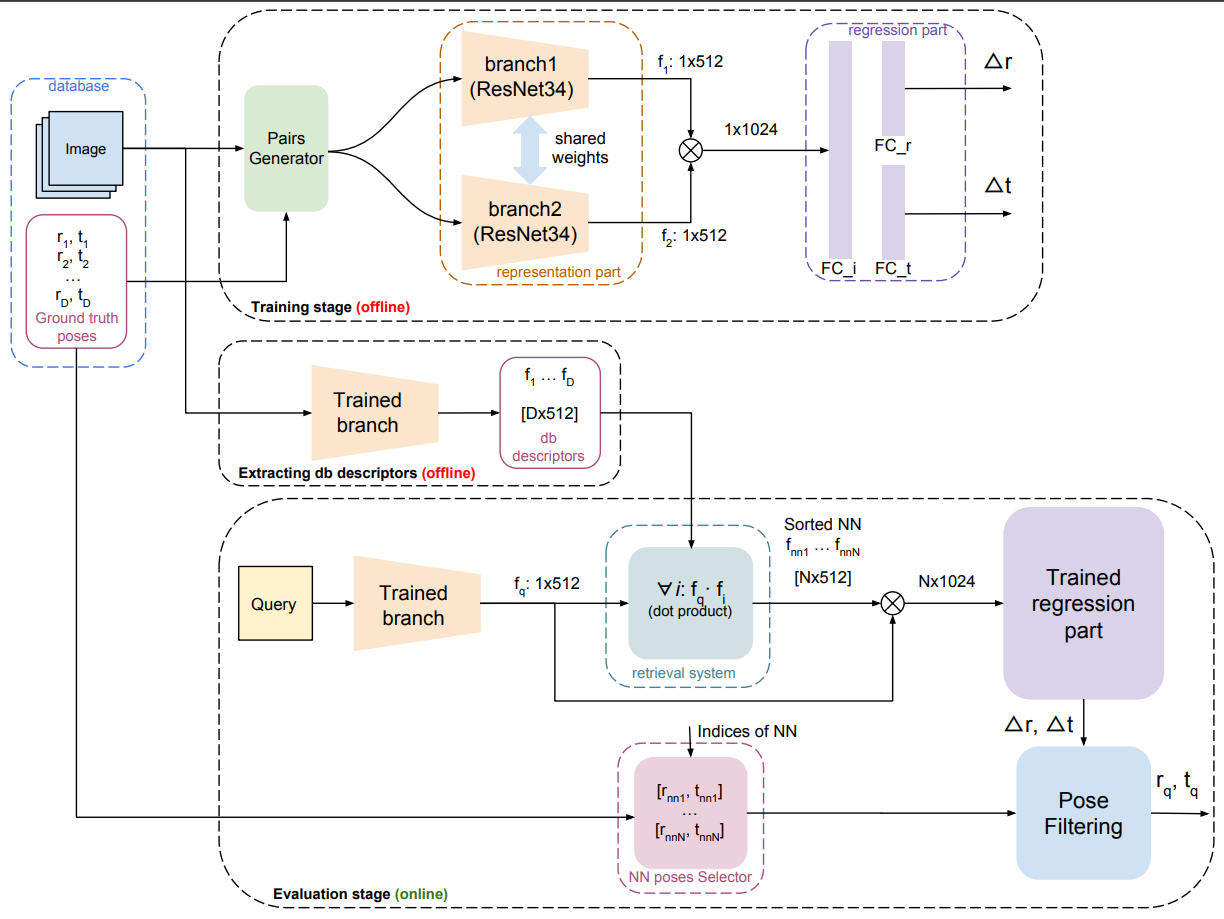
\includegraphics[width=0.7\textwidth]{pics/Chapter2/nnet.png}
    \caption{Minh họa kiến trúc mô hình NNet \cite{laskar2017camera}}
\end{figure}
RelocNet \cite{10.1007/978-3-030-01264-9_46} cải tiến NNet với việc học liên tục thước đo với mục đích học các đặc trưng ảnh toàn cục với một góc nhìn chóp cụt của máy ảnh để cải thiện kết quả, mất mát vị trí tương đối cũng được áp dụng. Mất mát vị trí tương đối học sự khác biệt vị trí giữa hai ma trận vị trí bằng cách sử dụng một biểu diễn ma trận cho hướng quay và độ dời vị trí. Hàm mất mát huấn luyện được định nghĩa như sau:
\begin{center}
$l = \alpha l_{SE(3)} + \beta l_{frustum}$
\end{center}
\begin{figure}[H]
    \centering
    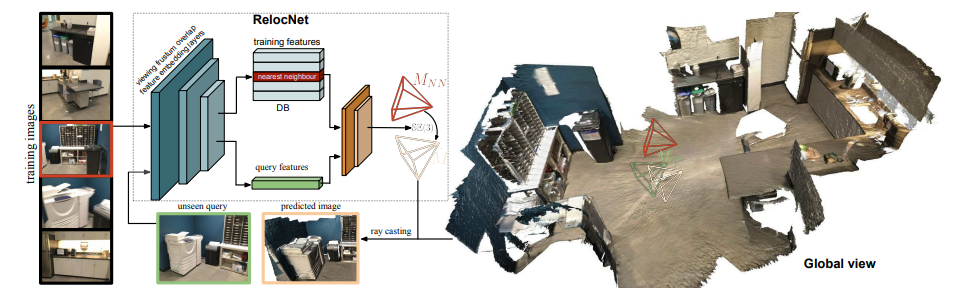
\includegraphics[width=\textwidth]{pics/Chapter2/relocnet.png}
    \caption{Minh họa kiến trúc mô hình RelocNet \cite{10.1007/978-3-030-01264-9_46}}
\end{figure}
Để giải quyết vấn đề hiệu suất giới hạn của các phương pháp hồi quy vị trí tương đối tiền nhiệm do sử dụng cùng đặc trưng cho cả hai bước truy xuất và hồi quy, CamNet \cite{9008579} đề xuất một quy trình chia làm ba bước: truy xuất thô, truy xuất mịn và hồi quy vị trí. Kiến trúc mô hình được xây dựng dựa trên kiến trúc Siamese với ba nhánh mỗi bước. Kiến trúc thô-sang-mịn này đã mang lại những cải tiến về hiệu suất hồi quy cũng như khả năng mở rộng. Hàm mất mát của CamNet lấy ý tưởng dựa trên RelocNet, được định nghĩa như sau:
\begin{center}
$l = l_{frustum} + l_{angle} + l_{triplet} + l_{PFR} + l_{PRP}$
\end{center}
\begin{figure}[H]
    \centering
    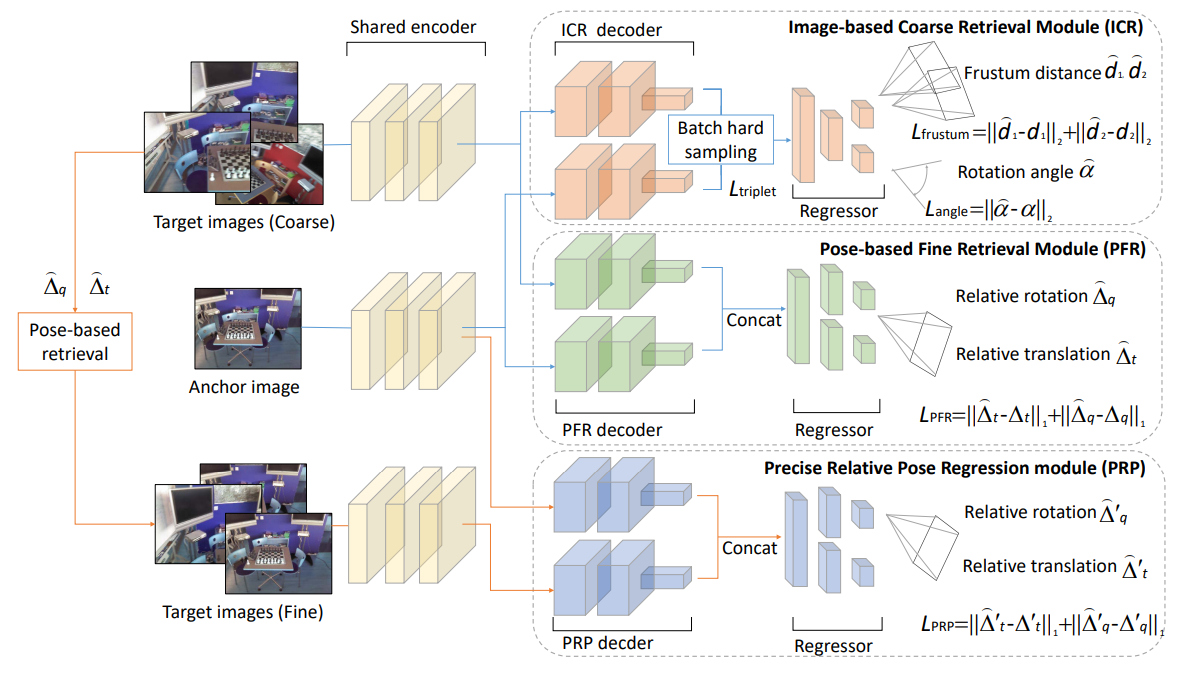
\includegraphics[width=0.7\textwidth]{pics/Chapter2/camnet.png}
    \caption{Minh họa kiến trúc mô hình CamNet \cite{9008579}}
\end{figure}
Qunjie Zhou và những cộng sự \cite{zhou2020learn} sau khi phân tích các phương pháp hồi quy vị trí dựa trên việc truy xuất ảnh đã đề xuất một kiến trúc mới sử dụng ma trận thiết yếu và RANSAC để tính toán vị trí tuyệt đối. Một mạng Siamese ResNet34 với một lớp tìm sự tương ứng cố định (EssNet) và một lớp tìm sự tương ứng đồng thuận lân cận (NC-EssNet) được học để tạo ra một bản đồ điểm tương ứng phục vụ cho mục đích hồi quy về sau của ma trận thiết yếu. Hàm mất mát cải tiến khoảng cách Euclidean giữa ma trận thiết yếu với hai véc-tơ 9 chiều.
\begin{center}
$l_{ess}(E^*, E) = \left \| e - e^* \right \|_2$
\end{center}
\begin{figure}[H]
    \centering
    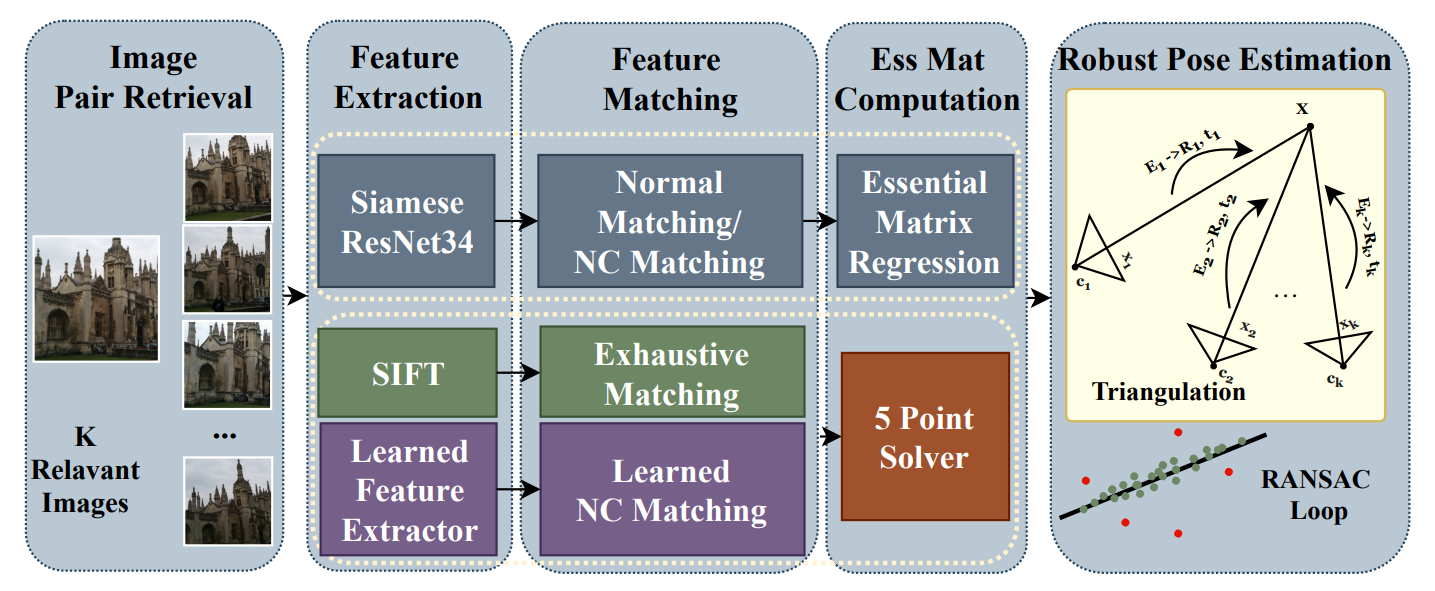
\includegraphics[width=0.7\textwidth]{pics/Chapter2/essnet.png}
    \caption{Minh họa kiến trúc mô hình EssNet \cite{zhou2020learn}}
\end{figure}

\subsubsection*{Hồi quy vị trí tương đối thông qua mạng CNN ngầm - Relative camera pose regression through implicit CNN}
Để tránh việc phải thu thập và xây dựng một kho dữ liệu khổng lồ cũng như tốn kém thời gian thử nghiệm, một số phương pháp tìm cách hồi quy vị trí tương đối của máy ảnh thông qua một mạng Nơ-ron tích chập ngầm.

Relative NN \cite{melekhov2017relative} đề xuất một phương pháp đầu-cuối để hồi quy vị trí tương đối giữa hai máy ảnh bằng hai ảnh đầu vào. Kiến trúc mô hình là một mạng Nơ-ron hỗn hợp Siamese hai nhánh sử dụng mạng AlexNet đã được huấn luyện từ trước được dùng cho việc hồi quy với hàm mất mát Euclidean cố định.
\begin{figure}[H]
    \centering
    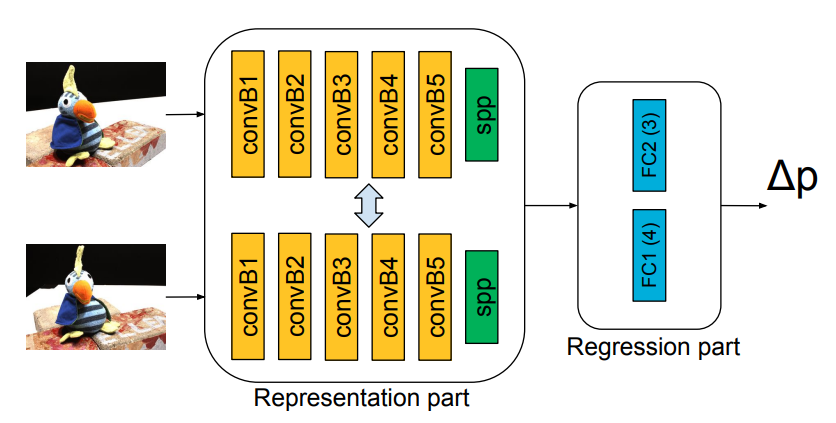
\includegraphics[width=0.7\textwidth]{pics/Chapter2/relativenn.png}
    \caption{Minh họa kiến trúc mô hình Relative Neural Network \cite{melekhov2017relative}}
\end{figure}
AnchorNet \cite{saha2018improved} tìm cách khắc phục vấn đề định vị bằng cách định nghĩa các địa danh thành các điểm mốc để học các điểm mốc tương đối của ảnh đầu vào cũng như độ lệch của chúng. Mô hình đa nhiệm bao gồm việc phân loại hình ảnh truy vấn đầu vào theo các điểm mốc cụ thể và tìm sự chênh lệch so với điểm mốc đã phân loại, điều này dẫn đến việc hình thành hàm mất mát. $\hat{C}$, $X$, và $Y$ đại diện cho kết quả phân loại và sự chênh lệch với sự thật nền tảng.
\begin{center}
$l = \sum_i[(X_i - \hat{X}_i)^2 + (Y_i - \hat{Y}_i)^2]\hat{C}^i$
\end{center}
\begin{figure}[H]
    \centering
    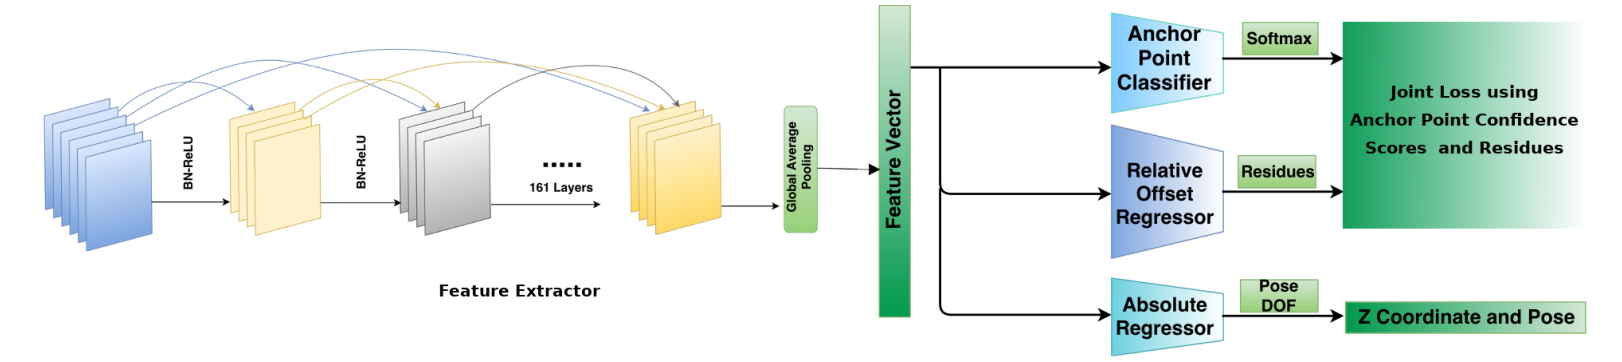
\includegraphics[width=0.7\textwidth]{pics/Chapter2/anchornet.png}
    \caption{Minh họa kiến trúc mô hình AnchorNet \cite{saha2018improved}}
\end{figure}

\subsubsection*{}
Nhận thấy các phương pháp tái định vị trực quan (Visual Relocalization) hiện tại đều cần một kho dữ liệu ảnh khổng lồ nhằm mục đích xây dựng một mô hình 3 chiều cho một khung cảnh nhất định, một nhóm nghiên cứu \cite{arnold2022mapfree} đề xuất phương pháp mang tên "Tái định vị không cần bản đồ (Map-free Relocalization)" với việc chỉ sử dụng duy nhất một ảnh làm đầu vào mà không cần phải xây dựng mô hình 3 chiều cho cảnh. \cite{arnold2022mapfree} đã đề xuất hai phương pháp khác nhau để có thể xác định vị trí, góc quay chính xác từ một ảnh: thứ nhất là tận dụng ma trận thiết yếu kết hợp với các kỹ thuật tìm sự tương ứng giữa đặc trưng ảnh, thứ hai là hồi quy vị trí tương đối.
\begin{figure}[H]
    \centering
    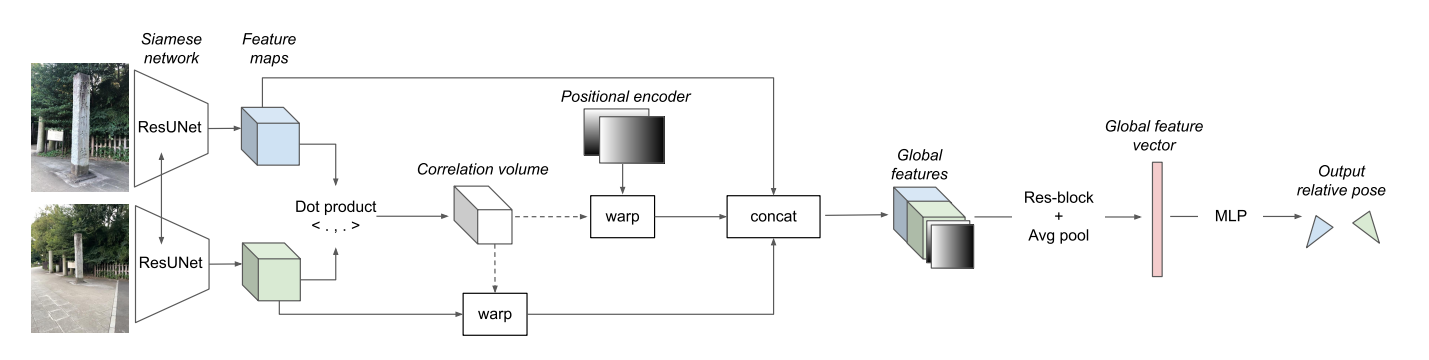
\includegraphics[width=0.7\textwidth]{pics/Chapter2/mapfreeRPR}
    \caption{Minh họa kiến trúc mô hình hồi quy vị trí tương đối của Map-free \cite{arnold2022mapfree}}
\end{figure}

\subsubsection*{Kết luận}
Để thực hiện tác vụ hồi quy vị trí tương đối, các phương pháp dựa trên truy xuất ảnh \cite{laskar2017camera, 10.1007/978-3-030-01264-9_46, 9008579, zhou2020learn} tận dụng một quy trình nhiều bước để lấy được vị trí tuyệt đối với bước truy xuất ảnh làm trọng tâm. NNnet \cite{laskar2017camera} là công trình đầu tiên đề xuất một phương pháp hồi quy vị trí tương đối dựa trên truy xuất ảnh, với RelocNet \cite{10.1007/978-3-030-01264-9_46} tìm cách cải tiến NNet với việc học liên tục thước đo với mục đích học các đặc trưng ảnh toàn cục kết hợp góc nhìn chóp cụt của máy ảnh để cải thiện kết quả. CamNet \cite{9008579} đề xuất một quy trình chia làm ba bước: truy xuất thô, truy xuất mịn và hồi quy vị trí với ba nhánh CNN mỗi bước và đã mang lại những cải tiến về hiệu suất hồi quy cũng như khả năng mở rộng. 

Trong khi đó các phương pháp dựa trên CNN \cite{melekhov2017relative, saha2018improved, arnold2022mapfree} lại đề xuất một hướng giải quyết để hồi quy trực tiếp vị trí tương đối ngay trong mạng nơ-ron. Relative NN \cite{melekhov2017relative} đề xuất một mô hình đầu-cuối Siamese hai nhánh để hồi quy vị trí tương đối giữa hai ảnh đầu vào. AnchorNet \cite{saha2018improved} tìm cách khắc phục vấn đề định vị bằng cách định nghĩa các địa danh thành các điểm mốc để học các điểm mốc tương đối của ảnh đầu vào cũng như độ lệch của chúng. Map-free \cite{arnold2022mapfree} đề xuất việc không sử dụng ảnh để tái kiến trúc lại cảnh, đồng thời cung cấp hai phương hướng để hồi quy vị trí từ một ảnh.


\subsection{Tái tạo kiến trúc từ chuyển động - Structure From Motion}

\section{Phân tích và tổng hợp}
Về các phương pháp hồi quy vị trí máy ảnh, các nghiên cứu cho thấy hiệu suất dự đoán vị trí vẫn chưa thể vượt qua các phương pháp tái kiến trúc từ chuyển động. Các phương pháp hồi quy vị trí máy ảnh vẫn còn đang trên đà phát triển tuy nhiên vẫn gặp nhiều khó khăn với việc giải quyết các đặc trưng cục bộ trùng lặp cũng như việc tiêu tốn nhiều tài nguyên tính toán. Hầu hết công trình tập trung vào các điểm đặc trưng có độ chắc chắn cao hoặc mô tả đặc trưng chính xác dưới điều kiện mang tính thử thách cao. Ngoài ra, phần lớn các phương pháp được đề xuất chỉ có thể áp dụng trong một phạm vi nhỏ và vẫn chưa chứng tỏ được hiệu suất trên những tập dữ liệu có quy mô lớn.
	
\section{Một số tập dữ liệu phổ biến được sử dụng}
\subsection{Tập dữ liệu trong không gian nhỏ}
\subsubsection*{7Scenes}
Tập dữ liệu 7-Scenes \cite{6619221} bao gồm các ảnh RGB-D thuộc bảy khung cảnh khác nhau được chụp từ một máy ảnh cầm tay Kinect RGB-D ở độ phân giải 640x480. Bảy khung cảnh bap gồm: "Chess", "Fire", "Heads", "Office", "Pumpkin", "RedKitchen" và "Stairs". Với mỗi cảnh sẽ có vài chuỗi khung ảnh RGB-D. Mỗi chuỗi bao gồm khoảng từ 1000 đến 5000 khung ảnh. Mỗi khung sẽ gồm: ảnh màu, độ sâu và vị trí.
\begin{figure}[H]
    \centering
    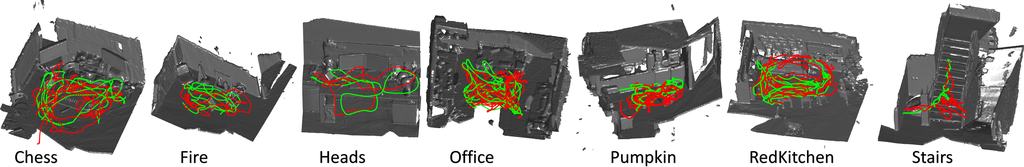
\includegraphics[width=\textwidth]{pics/Chapter2/7scenes.png}
    \caption{Minh họa tập dữ liệu 7-Scenes \cite{6619221}}
\end{figure}
\subsubsection*{Cambridge Landmark}
Tập dữ liệu Cambridge Landmarks \cite{kendall2016posenet} là một tập dữ liệu định vị thành thị bao gồm năm khung cảnh khác nhau. Các yếu tố dày đặc quan trọng như phương tiện giao thông hay người đi bộ cũng xuất hiện trong tập dữ liệu này, ngoài ra dữ liệu cũng được thu thập ở nhiều thời điểm trong ngày đại diện cho các yếu tố ánh sáng và điều kiện thời tiết khác nhau. Cambridge Landmarks được tạo ra nhờ vào việc áp dụng các kỹ thuật tái tạo kiến trúc từ chuyển động. Một chiếc điện thoại thông minh Google LG Nexus 5 được một người đi bộ trên phố sử dụng để ghi lại đoạn phim chất lượng cao cho mỗi cảnh. Mỗi đoạn phim sau đó sẽ được lấy mẫu với tần số 2Hz để trích xuất ảnh cho quy trình tái tạo kiến trúc từ chuyển động. Mỗi vị trí máy ảnh sẽ cách nhau khoảng 1m.
\begin{figure}[H]
    \centering
    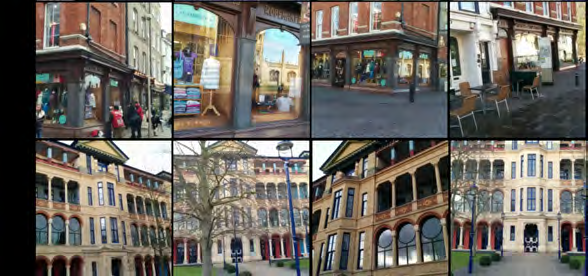
\includegraphics[width=\textwidth]{pics/Chapter2/cambridge.png}
    \caption{Minh họa tập dữ liệu Cambridge Landmarks \cite{kendall2016posenet}}
\end{figure}
\subsubsection*{Niantic Map-free Relocalization Dataset}
Tập dữ liệu Niantic Map-free Relocalization \cite{arnold2022mapfree} là một tập dữ liệu được thu thập chủ yếu để giúp ích cho phương pháp định vị Map-free \cite{arnold2022mapfree}. Tập dữ liệu bao gồm 655 cảnh bên ngoài với mỗi cảnh sẽ chứa một "địa điểm đáng chú ý" như một pho tượng, cổng, bảng hiệu,... sao cho địa điểm đó phải được xác định rõ trong một bức ảnh. Các cảnh được chia ra thành 460 cảnh phục vụ cho tác vụ huấn luyện, 65 cảnh phục vụ cho tác vụ kiểm tra quy trình huấn luyện và 130 cảnh phục vụ cho quá trình kiểm thử. Mỗi ảnh trong tập huấn luyện đều được gắn kèm vị trí tuyệt đối. Với tập kiểm thử và kiểm tra quy trình, mỗi cảnh sẽ được kèm theo một ảnh đại diện cũng như vị trí tuyệt đối tại cảnh. Ngoài ra, ma trận tham số nội tại của máy ảnh cũng được gắn kèm theo mỗi ảnh trong tập dữ liệu.
\begin{figure}[H]
    \centering
    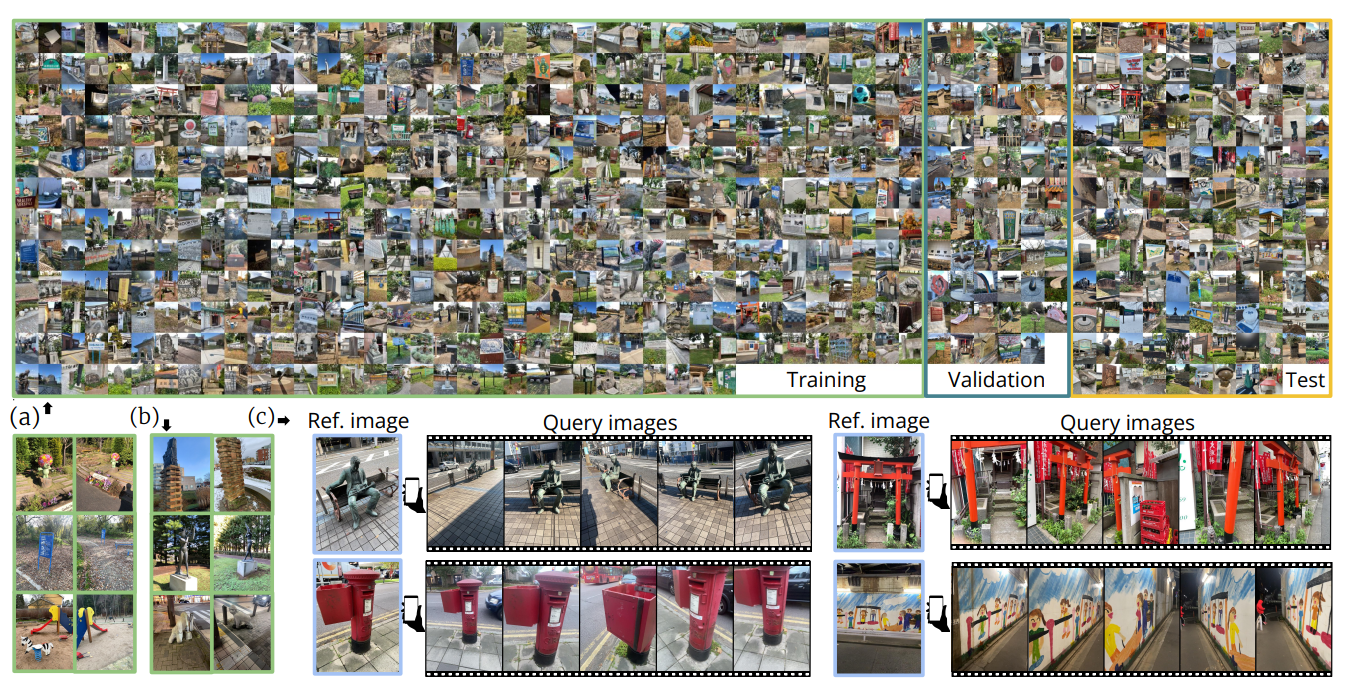
\includegraphics[width=\textwidth]{pics/Chapter2/niantic.png}
    \caption{Minh họa tập dữ liệu Niantic Map-free Relocalization \cite{arnold2022mapfree}}
\end{figure}
\subsection{Tập dữ liệu thành thị}
\subsubsection*{Aachen Day-Night}
Tập dữ liệu Aachen Day-Night \cite{Sattler2012ImageRF} bao gồm 14.607 ảnh được chụp với nhiều máy ảnh khác nhau bao phủ cả thành phố Aachen thuộc quốc gia Đức. Các ảnh dữ liệu được chụp ở nhiểu thời điểm trong ngày và trong năm, cụ thể là khoảng thời gian trong 2 năm. Hệ quả mang lại là tập dữ liệu bao phủ nhiều điều kiện ngoại cảnh như thời tiết, ánh sáng cũng như sự thay đổi của công trình kiến trúc trong khu vực.
\begin{figure}[H]
    \centering
    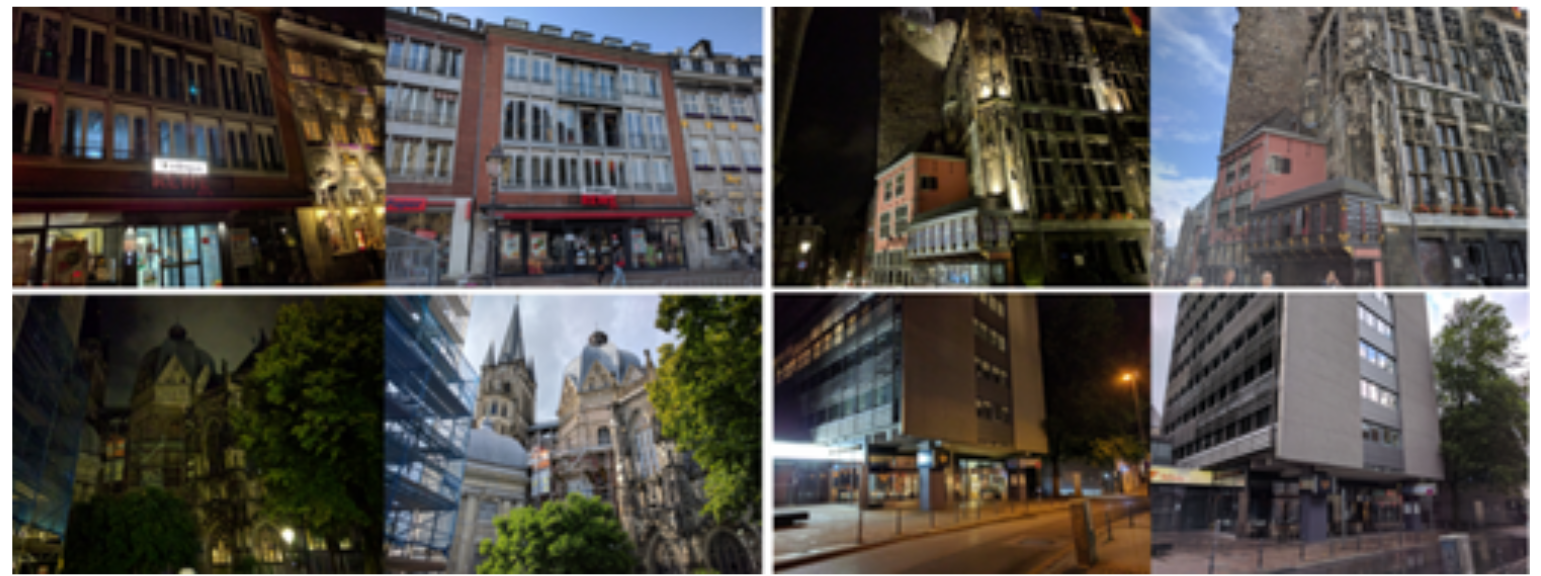
\includegraphics[width=\textwidth]{pics/Chapter2/aachen.png}
    \caption{Minh họa tập dữ liệu Aachen Day-Night \cite{Sattler2012ImageRF}}
\end{figure}
\subsubsection*{Pittsburgh 250k}
Tập dữ liệu Pittsburgh 250k \cite{6618963} là một tập dữ liệu tương đối rộng bao phủ thành phố Pittsburgh của Mỹ. Đây là một tập dữ liệu tương đối phổ biến trong thị giác máy tính, cụ thể là ở tác vụ nhận điện địa điểm trực quan, truy xuất ảnh và định vị trực quan.

\subsubsection*{GSV-Cities}
Tập dữ liệu GSV-Cities \cite{Ali_bey_2022} bao phủ một vùng địa lý cực kỳ rộng lớn với hơn 40 thành phố xuyên lục địa trong khoảng thời gian 14 năm liên tục. GSV-Cities chứa khoảng hơn 530.000 ảnh - khoảng hơn 62.000 vị trí. Mỗi vị trí sẽ có khoảng từ 4 đến 20 ảnh. Đồng thời mỗi vị trí sẽ cách nhau một khoảng ít nhất 100m.
\begin{figure}[H]
    \centering
    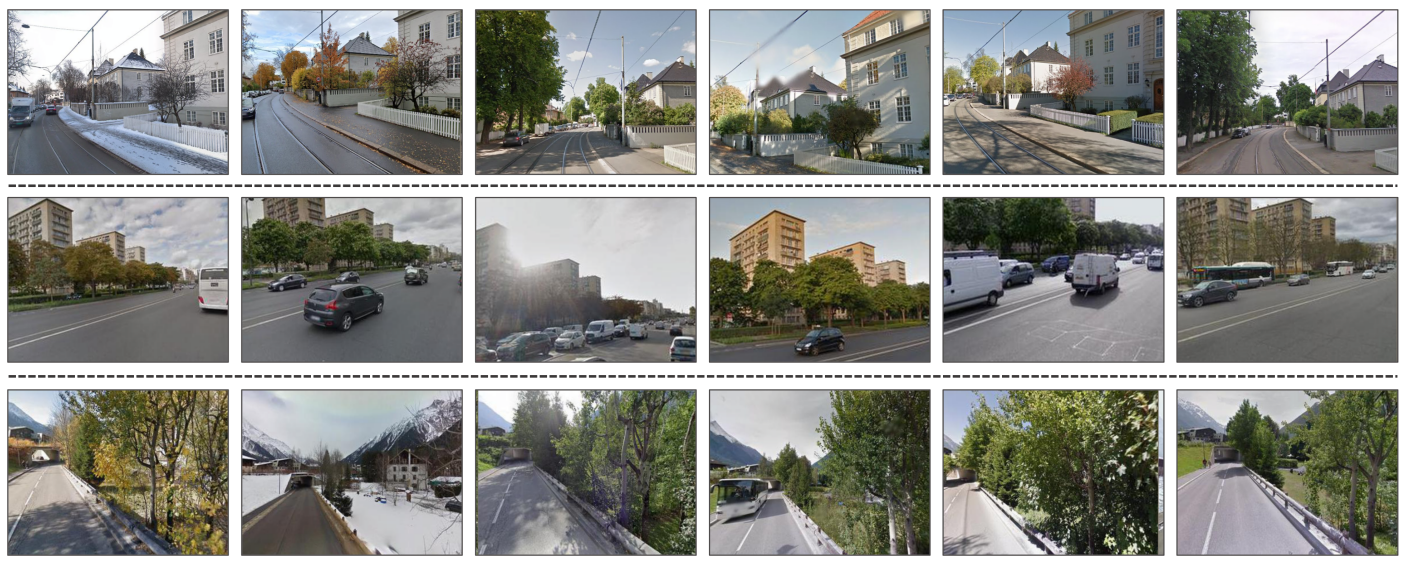
\includegraphics[width=\textwidth]{pics/Chapter2/gsv.png}
    \caption{Minh họa tập dữ liệu GSV-Cities \cite{Ali_bey_2022}}
\end{figure}

\subsubsection*{SF-XL}
Tập dữ liệu San Francisco Extra Large (SF-XL) \cite{berton2022rethinking} được tạo nên từ 3.43 triệu ảnh 360 độ thu thập từ kho ảnh Google Streetview. Các ảnh này sau đó được cắt ra thành 41.2 triệu ảnh. Mỗi ảnh cắt ra đều được gắn nhãn 6DoF (bao gồm cả GPS). Dữ liệu được thu thập từ năm 2009 đến năm 2021, dẫn đến việc tập dữ liệu bao phủ nhiều điều kiện ngoại cảnh như thời tiết, ánh sáng cũng như sự thay đổi của công trình kiến trúc trong khu vực.
\begin{figure}[H]
    \centering
    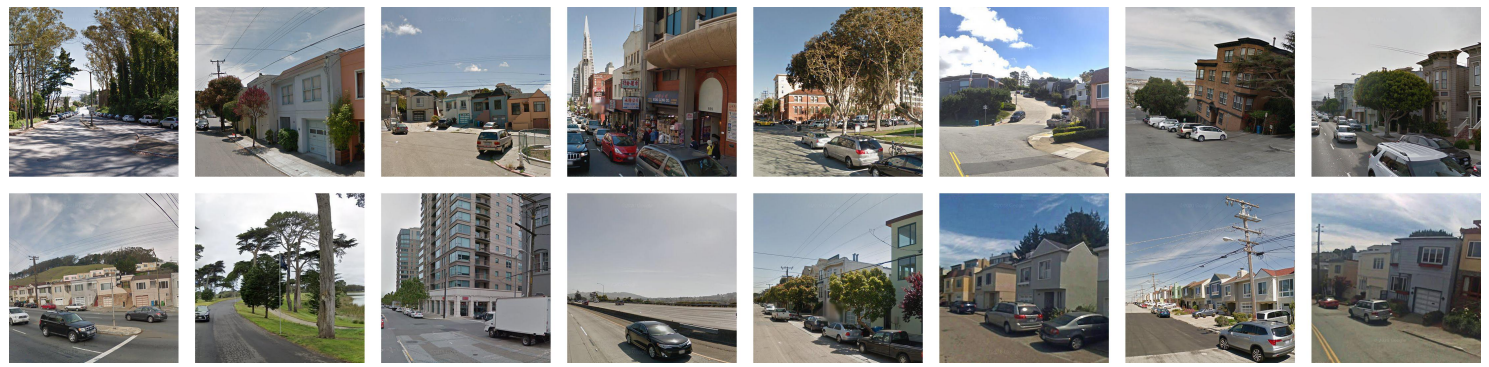
\includegraphics[width=\textwidth]{pics/Chapter2/sfxl.png}
    \caption{Minh họa tập dữ liệu San Francisco Extra Large \cite{berton2022rethinking}}
\end{figure}

